\documentclass[logo,civil]{tesis-pregrado}
%opciones: logo,dosdirectores,civil,ejecucion,propuesta,txfonts
\usepackage{float,lscape, booktabs}
\keywords{XML; Social Networks}

\begin{document}

\baselineskip 23pt

% ----------------------------------------------------------
% ----------- PARTE INICIAL --------------------------------
\thispagestyle{empty}

\titulo{Detección de Comunidades en los Sistemas de Recomendación: Uso de una Caché en Rbox 2.0.}

\autor{Juan Alberto Daniel Ochoa John}
\email{juan.ochoa@usach.cl}
\telefono{7898 1877}
\run{17.405.225\-5}
\annoingreso{2012}

\fecha{Lunes}{21}{Junio}{2014} %Lunes 30 de Mayo de 2011

\director{Dr.\ Edmundo Leiva Lobos}

\ciudad{Santiago}
\pais{Chile}

\makecubierta

% \thispagestyle{empty}
% 
\titulo{Detección de Comunidades en los Sistemas de Recomendación: Uso de una Caché en Rbox 2.0.}

\autor{Juan Alberto Daniel Ochoa John}
\email{juan.ochoa@usach.cl}
\telefono{7898 1877}
\run{17.405.225\-5}
\annoingreso{2012}

\fecha{Lunes}{11}{Junio}{2012} %Fecha de defensa Lunes 30 de Mayo de 2011

\director{Dr.\ Edmundo Leiva Lobos}
\regular{Dr.\ Edmundo Leiva}
\regular{Mag.\ Javier Jara}


\ciudad{Santiago}
\pais{Chile}

\makecaratula

\makecopyright
\newpage
\mbox{}
\thispagestyle{empty}
% ----------------------------------------------------------
% ----------- PRIMERA PARTE --------------------------------
\frontmatter
% ### Resumen e Indices ####

\begin{gracias}
Gracias a todos.
\end{gracias}


\dedicatoria{
  A mi incondicional familia y a mi fant\'astica mujer, esto no habr\'ia sido posible sin ustedes\ldots
}

\resumenCastellano{

El objetivo de esta tesis es verificar si precomputar comunidades mejora la eficiencia de los sistemas de recomendación (SR). Los SR entregan recomendaciones como salida, con el fin de presentar a un usuario activo un conjunto de opciones de su interés, basado en distintos aspectos, uno de ellos son las comunidades a las que el usuario pertenece. La tesis se ha apoyado en un \textit{framework} de eventos colaborativos llamado 3-Ontology, implementado en una API denominado Rbox 2.0 donde la comunidad es una de sus dimensiones esenciales.

Las interacciones entre usuarios y aplicaciones en la Web 2.0 hacen emerger comunidades. Los seguidores de \textit{Twitter} de un usuario forman una comunidad, los que han comprado un mismo libro en \textit{Amazon} también. Los SR hacen uso de comunidades, y típicamente es preciso usar estrategias para detectarlas. No obstante, estas estrategias no están apoyadas por un mecanismo que soporte el proceso de recomendación íntegramente y sus resultados deben ser reprocesados cada vez al momento de computar una recomendación. El contar con un \textit{framework} que estandariza la representación de la información de las distintas interacciones que ocurren en plataformas basadas en la Web 2.0, permite que la detección de comunidades pueda ser realizada de manera estándar. Como añadidura a RBox, se ha construído un mecanismo de abstracción, representación, detección y persistencia - \textit{community cache} - que permite contar con un respaldo de las comunidades ya detectadas en recomendaciones anteriores.

Para validar la eficacia del modelo propuesto, se ha desarrollado un sistema de recomendación, que utiliza el modelo, y recomienda en base a distintas estrategias de detección de comunidades existentes en la literatura. Los escenarios de prueba definidos, muestran que el tiempo promedio necesario para recomendar utilizando la información de las comunidades detectadas con el apoyo del modelo construido es hasta un 7\% menor que cuando se realiza el mismo ejercicio sin él. Como aporte al área de SR, se provee una capa de abstracción al \textit{framework} RBox, que permite detectar, persistir y utilizar en la recomendación, información respecto a las comunidades emergentes de manera eficiente.

\vspace*{0.5cm}

\KeywordsES{\textit{community detection}, Sistemas de Recomendación, Web 2.0, 3-Ontology, \textit{community cache}, \textit{social networking}}

}

\resumenIngles{

The main objective of this thesis is verify if the efficiency of recommendation systems (RS) improves when the communities are pre calculated. The output of RS are recommendations presented to an active user and intends to guide his navigation on contents of their interest. Recommendations are based on different aspects, one of those aspects are the communities to the user belongs. This thesis has been supported on a framework of collaborative events called 3-Ontology, implementing an API called RBox 2.0, where the communities are one of the essentials dimensions.

The result of the interactions between users and Web 2.0 applications is the apparition of many communities. The Twitter followers of an user forms a community as well as the buyers of a same book on Amazon. The RS  uses communities and typically different detection strategies are needed to identify them. However, those strategies are not backed on a mechanism that entirely supports the recommendation process, and the detection results must be reprocessed in every recommendation. The fact of counting with a framework that standardizes the representation of every interaction produced in a social media environment permits that the community detection may be realized in a standard way. As a plugin to RBox, we present a mechanism of community abstraction, representation, detection and persistence (community cache), that permits handling a backup of the communities that have been already detected in past recommendations.

In order to validate the efficacy of the proposed model, we have developed a recommendation system, that uses the model, and performs recommendations based on different community detection strategies, based on literature. The testing scenarios show that the average recommendation time is seven percent lower when the recommendations are performed with the proposed model. As a contribution to the RS area, we present an abstraction layer for the Rbox framework, that permits to detect, persist and use efficiently in the recommendation, the information related to different emerging communities.

\vspace*{0.5cm}

\KeywordsEN{community detection, recommendation systems, Web 2.0, 3-Ontology, community cache, social networking}
}

\pagestyle{fancy}
\fancyhead[L]{\slshape \leftmark}
\fancyhead[C]{}
\fancyhead[R]{\thepage}
\tableofcontents        %% Indice general
\listoffigures          %% Indice de figuras
\listoftables           %% Indice de tablas
%\listofalgorithms       %% Indice de algoritmos

% ----------------------------------------------------------
% ----------- SEGUNDA PARTE --------------------------------
\mainmatter
% ### Configuración del header ###
\pagestyle{fancy}
\fancyhead[L]{\slshape \leftmark}
\fancyhead[C]{}
\fancyhead[R]{\thepage}
\pagenumbering{arabic}

% ### Capitulos de la tesis ###
%--------Introducción
%--------Daniel Ochoa John
%--------19/07/2014

\chapter{Introducci\'on}
\label{cap:intro}

El objetivo de este capítulo es presentar el problema y la propuesta de la solución de la detección de comunidades emergentes desde las interacciones sociales en la Web 2.0 usando el \textit{framework} de eventos de la 3-Ontology. La propuesta es incorporar la dimensión de la comunidad en el \textit{framework} para crear sistemas de recomendación llamado RBox.

\section{Antecedentes y motivaci\'on}
\label{intro:motivacion}

Vivimos en un mundo donde la cotidianidad ha sido invadida por distintos aparatos tecnológicos inteligentes, que han permitido a las personas acceder a la Web en cualquier momento y en cualquier lugar. Esto, sumado a la envolvente aparición de la Web 2.0, implica que los usuarios de Internet ya no solo se dedican a consumir información, sino que, muy por el contrario, ahora asumen roles como actores determinantes en la generación de contenidos (Andersen, 2007). Ciertamente, las barreras que antes existían entre ser productor y consumidor de información han caído, empoderando a los usuarios a ser un agente activo en el flujo de la información. La Web 2.0, en definitiva, ha propiciado una forma diferente de usar la Web como canal de comunicación (Padula, Reggiori, & Capetti, 2009).

El uso masivo de aplicaciones móviles, Web y todo tipo de aplicaciones sociales en general ha provocado que Internet almacene una enorme cantidad de información. Esto ha generado un problema para los millones de usuarios de la Web, ya que es complejo acceder a información que sea acorde con los gustos e intereses particulares para cada uno de ellos. En ese sentido, el asistir a los usuarios de Internet a filtrar y discriminar información relevante, ha sido una de las principales motivaciones de investigadores de las ciencias de la información, principalmente enfocándose en dos grandes áreas: los motores de búsqueda y los sistemas de recomendación.  Estos últimos filtran la información de acuerdo a distintas dimensiones (Adomavicius & Tuzhilin, 2011), como la confiabilidad y el prestigio de los usuarios (Victor, De Cock, & Cornelis, 2011), geolocalización (Symeonidis, Papadimitriou, Manolopoulos, Senkul, & Toroslu, 2011) y el contexto de interacción (Adomavicius & Tuzhilin, 2011) y a una serie de directrices, que van desde el comportamiento de otros usuarios, preferencias explicitadas en el pasado propias, ajenas y aquellas tipificadas por las comunidades en las que un usuario participa (Arab & Afsharchi, 2014).

Comunidades online como \textit{Twitter}, \textit{Facebook} y \textit{YouTube} han tenido un crecimiento notable durante los últimos años, e incluso son posicionados entre los sitios más visitados de Internet. En estas plataformas, los usuarios pueden crear, explorar y compartir de diversas formas (Brambilla, Fraternali, & Vaca, 2011) con distintos grupos de manera explícita, como en \textit{Facebook} o Google+ o implícita, como en \textit{Twitter}.  Una manera de explicitar las comunidades existentes en un entorno colaborativo social es mediante la detección de comunidades (en inglés, \textit{community detection}). Una comunidad típicamente se define como un conjunto de individuos que tienen propiedades en común (Du, Wu, Pei, Wang, & Xu, 2007) y para detectarlas existen diversas técnicas y algoritmos (Plantié & Crampes, 2013).

Las aplicaciones de la detección de comunidades son diversas. Entre ellas se puede encontrar el análisis temporal de las comunidades online, como los bloggers o los sistemas de recomendación de medios digitales (Lin, Sundaram, Chi, Tatemura, & Tseng, 2007; Schlitter & Falkowski, 2009), en donde interesa conocer las correlaciones temporales entre los usuarios y sus relaciones. Además, es posible conocer los tipos de transformaciones (Palla, Barabási, Vicsek, & Hungary, 2007) que tiene una comunidad en el tiempo: compresiones, contracciones y divisiones. Es posible, también, analizar la detección de tópicos en sistemas de etiquetado colaborativos, para detectar los temas más relevantes que son tocados al interior de una comunidad, en base a taxonomías o folksonomías (Simpson, 2008; Papadopoulos, Kompatsiaris, & Vakali, 2009). Por lo que es relevante contar con la información de las comunidades al momento de realizar una recomendación.

\section{Descripci\'on del problema}
\label{intro:problema}

En un contexto de interacción social se forman diversas comunidades de usuarios en base a distintos intereses o temas. Esas comunidades no siempre están visibles ni disponibles para su uso en las aplicaciones de la Web 2.0. Además, estas comunidades pueden estar de manera latente y en respuesta a contenido recientemente popular y son información que los sistemas de recomendación podrían utilizar para mejorar su desempeño.

En concreto, al momento de generar una recomendación, es necesario procesar y detectar cada vez esas comunidades latentes, con la implicancia de que en cada ejecución del algoritmo de recomendación se destinen recursos computacionales a detectar comunidades que ya han sido identificadas en iteraciones anteriores, aumentando innecesariamente el tiempo de respuesta necesario para otorgar una recomendación. Luego, la pregunta de investigación precisa de esta tesis es la siguiente: ¿es posible mejorar el desempeño de los sistemas de recomendación pre computando de comunidades implicadas en la recomendación?.

\section{Soluci\'on propuesta}
\label{intro:solucion}

Este proyecto de investigación es del tipo Investigación Aplicada I+D (Investigación y Desarrollo):

\begin{enumerate}
  \item \textbf{Investigación:} Como hipótesis científica, este trabajo plantea que contar con un mecanismo de \textit{‘cache’} para manejar las comunidades detectadas en ejecuciones previas de un sistema de recomendación, permite mejorar el tiempo de respuesta necesario para otorgar una recomendación.
  \item \textbf{Desarrollo:} Se diseñará y construirá una arquitectura orientada a servicios, que faculte a RBox 2.0 (Vasquez, 2014) a manejar la detección de comunidades y la construcción de sistemas de recomendación que consideren a esta dimensión dentro de la 3-Ontology.
\end{enumerate}

\subsection{Caracter\'isticas de la Soluci\'on}

Las características de la solución son las siguientes:

\begin{itemize}
  \item Un componente de \textit{software} que hace uso del API que provee RBox, basado en patrones de diseño acordes con la implementación ya realizada.
  \item Un sistema orientado a servicios que posibilite la detección de comunidades aplicando diferentes enfoques.
  \item La disponibilización de un dataset inédito, que será utilizado como base para su mapeo al esquema 3-Ontology.
  \item Prueba de tiempo de ejecución aplicando distintos métodos de detección de comunidades, en un sistema de recomendación generado con RBox.
\end{itemize}

\subsection{Prop\'osito de la Soluci\'on}

\begin{itemize}
  \item Proveer un componente de \textit{software} extensible, cuyo foco sea el análisis de comunidades y, en particular, la detección de comunidades.
  \item Añadir a la arquitectura de RBox un componente de \textit{software} que sea capaz de consumir este servicio, permitiendo así la implementación de procedimientos que hagan uso de la dimensión comunidad.
  \item Extender la herramienta RBox, otorgando al área de los SR una herramienta que se empodera cada vez más en el uso del darse-cuenta colaborativo en el esquema basado en eventos propuesto por Leiva-Lobos y Covarrubias (2002).
\end{itemize}

\section{Objetivos y alcance del proyecto}
\label{intro:objetivos}

A continuación se presenta el objetivo general del proyecto, el cual se lleva a puerto a través del cumplimiento de los diversos objetivos específicos. Además, se declaran los alcances del trabajo de tesis.

\subsection{Objetivo general}

Detectar comunidades implícitas que se forman a través de las interacciones de los usuarios en la Web social para conseguir sistemas de recomendación más eficientes utilizando el \textit{framework} que provee Rbox 2.0.

\subsection{Objetivos espec\'ificos}


\begin{enumerate}
  \item Seleccionar técnicas y/o algoritmos que permitan la detección de comunidades.
  \item Definir la arquitectura del servicio que se añadirá a RBox 2.0, junto con un proceso de encapsulamiento de los datos del \textit{framework} para estandarizar el consumo del servicio.
  \item Implementar y añadir a RBox 2.0 un servicio que detecte y persista las comunidades (\textit{community cache}) a partir de los datos encapsulados.
  \item Implementar un algoritmo de recomendación utilizando la información de las comunidades como antecedente, para registrar el tiempo de respuesta requerido para entregar una recomendación.
  \item Analizar tiempos de respuesta obtenidos al monento de generar recomendaciones, con la finalidad de confirmar o descartar la hipótesis planteada.
  \item Desarrollar conclusiones en relación a los resultados obtenidos.
  \item Publicar los resultados en una revista de la especialidad.
\end{enumerate}

\subsection{Alcances}

El trabajo de tesis propuesto tiene los siguientes alcances:

\begin{itemize}
  \item Contempla solamente la dimensión de la comunidad de la 3-Ontology y en particular, la detección de comunidades.
  \item Se basa  en la definición de SR y alcances establecidos en la tesis de Magíster de Vásquez (2014).
  \item Solamente se validará con el dataset generado, y que está basado en la red social \textit{Twitter}, no obstante todos los modelos realizados serán genéricos, para cualquier red social.
  \item El producto de \textit{software} será construído en base a las definiciones y estándares ya definidos en RBox.
  \item La implementación del servicio de análisis de comunidades será de tipo RESTful y será independiente de RBox.
  \item La implementación de componentes para RBox hereda las limitantes y alcances ya definidos respecto al entorno de ejecución.
\end{itemize}

\section{Metodolog\'ia y herramientas de desarrollo}
\label{intro:metodologia}

\subsection{Metodolog\'ia}
La metodología usada para este trabajo, como se explicó anteriormente, tiene que ver en el contexto de un proyecto de investigación aplicado I+D.

En el ámbito de la investigación se realizará una prueba empírica respecto del tiempo de ejecución de un sistema de recomendación, bajo una estrategia de comienzo en frío (Lam, Vu, Le, & Duong, 2008), y que considere la dimensión de la comunidad. El proceso y el detalle involucrado en la recomendación y en la detección de comunidades propiamente tal será detallado en el Capítulo \ref{cap:arquitectura}.

En el ámbito del desarrollo, la metodología de desarrollo está basada en la filosofía ágil de SCRUM. Sin roles explícitamente definidos al tratarse de un trabajo personal. La necesidad de la agilidad tiene que ver con la volatilidad de los requerimientos y las variaciones sobre la marcha en la arquitectura, luego y de esta forma, se tiene la flexibilidad suficiente para abordar cambios a lo largo del desarrollo. La documentación que se genera es la mínima indispensable:

\begin{itemize}
  \item Documentación del código mediante Javadocs.
  \item Diseño de arquitectura.
\end{itemize}

\subsection{Herramientas de desarrollo}

Las herramientas que fueron usadas para la realización de este trabajo de tesis son las siguientes:

\begin{itemize}
  \item \textbf{Linux/Elementary OS Luna y Mac OSX 10.9.3}, como soportes del ambiente de desarrollo.
  \item \textbf{Java SE Development Kit 7}, para el desarrollo del \textit{software}. Su uso hereda de la decisión tomada en el desarrollo de RBox, basándose en la extensibilidad definida en la herramienta.
  \item \textbf{Sublime Text 2/3 y Netbeans IDE}, como apoyo al desarrollo de las aplicaciones.
  \item \textbf{Bitbucket}, como repositorio de código GIT.
  \item \textbf{Python 2.7 y Flask}, como entornos de desarrollo del servicio RESTful.
  \item \textbf{igraph}, como librería especializada en el análisis de grafos.
  \item \textbf{TeXstudio}, como herramienta para la construcción de documentos en LaTeX.
  \item \textbf{Notebook MacBook Pro Mid 2012}, Intel Core i5 2.5 GHz, 4 GB 1600 MHz DDR3.
  \item \textbf{Notebook Lenovo Ideapad Y500}, Intel Core i7 3630QM (2400 MHz - 3400 MHz), 8 GB 1600 MHz DDR3.
\end{itemize}

\section{Resultados Obtenidos}
\label{intro:resultados}

Se ha definido un \textit{framework} compuesto de una arquitectura orientada a servicios y un componente de \textit{software} añadido a RBox. Estas piezas de \textit{software}, permiten realizar una detección de comunidades a partir de un grafo de interacciones sociales para luego retroalimentar el esquema de 3-Ontology con las comunidades detectadas a partir de recomendaciones realizadas. Esto permite que, al volver a generar una recomendación similar, el tiempo de ejecución necesario para que esta recomendación se complete se reduzca, mediante el uso de una estrategia de persistencia (\textit{community cache}).

\section{Organizaci\'on del documento}
\label{intro:organizacion}

El documento se organiza como sigue. En el Capítulo 2 se presenta un marco teórico en donde se exponen los fundamentos conceptuales del trabajo, como detección de comunidades, la 3-Ontology y la descripción de los trabajos realizados anteriormente en el equipo de desarrollo de la universidad. Como antecedente del desarrollo de la solución presentada en esta tesis, en el Capítulo 3 se analizan los distintos componentes que dan forma a la plataforma tecnológica que apoya la experimentación requerida para alcanzar el objetivo general. Luego, en el Capítulo 4, se presenta el primer componente de \textit{software} desarrollado como producto de este trabajo: un servicio para la detección de comunidades. Posteriormente, en el Capítulo 5, se describe arquitecturalmente un componente de \textit{software} que integra a RBox el servicio de detección de comunidades y permite la persistencia y retroalimentación de las comunidades detectadas a partir de una recomendación. En el Capítulo 6 se describe y muestran los resultados del experimento definido para evidenciar el cumplimiento del objetivo general que este trabajo de tesis plantea. Finalmente, en el Capítulo 7 se presentan las conclusiones obtenidas a partir de este trabajo.

%--------Marco Teórico
%--------Daniel Ochoa John
%--------20/07/2014
\renewcommand{\thefigure}{\thechapter-\arabic{figure}}

\chapter{Marco Teórico}

\label{cap:marcoteorico}

En este capítulo se exponen los fundamentos teóricos del trabajo de tesis. Primero, se define el concepto de red social y sus formas de representación. Luego, se explora el concepto de análisis de redes sociales orientado principalmente a la detección de comunidades. Posteriormente, se define el concepto de sistema de recomendación, analizando aquellos conceptos que son considerados en este trabajo de tesis. Finalmente, se describe la lógica de la 3-Ontology, junto con un repaso de lo realizado anteriormente en relación a este concepto.

\section{Redes Sociales}

Las relaciones interpersonales son básicas para todo ser humano y están presentes en nuestra vida cotidiana, interactuamos con personas a cada momento y en cada lugar. Sociológicamente hablando, es posible definir el concepto de relación interpersonal como el total de interacciones que generan las personas en un contexto determinado (Dalton, 2007).

Estas interacciones pueden presentarse en distintos ámbitos, como por ejemplo, personales o laborales. Si se abstrae este concepto de relación interpersonal, es posible compararlo al contexto actual en lo que se conoce como una red social. Una red social es una estructura compuesta por nodos (individuos u organizaciones) y aristas, que conectan a los nodos formando una relación. Dichas relaciones pueden deberse a distintos tipos de interacciones como amistad, interés, entre otras.

Existen métodos para la representación de redes sociales, no obstante típicamente son utilizados dos. Uno es gráficamente mediante el renderizado de un grafo, otro es a través de una matriz de adyacencia (Wasserman & Faust, 1994). Las aristas en las redes sociales pueden contener distintos atributos, como peso, signo y dirección. Cuando las aristas contienen peso, es que a ellas se ha asociado un valor numérico que mide la relación en cierto aspecto (calidad, cercanía, similitud, entre otros), el signo puede determinar si la relación entre dos nodos es positiva o negativa, finalmente la dirección indica el sentido en el que la relación está definida.

\section{An\'alisis de Redes Sociales}

Las redes sociales en un contexto de \textit{social media} son generalmente muy grandes, con millones de usuarios y conexiones entre ellos. Haciendo uso de las capacidades únicas de masividad que provee la \textit{social media}, estas redes están presentando desafíos con respecto a su análisis (Tang & Liu, 2010):

\begin{enumerate}[I]
	\item \textbf{Escalabilidad:} Las redes sociales pueden crecer a tamaños astronómicos, conteniendo cientos de miles de conexiones. En \textit{Facebook}, por ejemplo, es tan evidente como que la comunidad de fans del fútbol tiene un orden de magnitud de 500 millones de usuarios (Smith, 2014). El análisis de redes sociales clásico tradicionalmente maneja un orden de magnitud de cientos o menos.
	\item \textbf{Heterogeneidad:} Entre dos usuarios puede existir múltiples tipos de relaciones. En la red social Google+, se aborda este concepto a través del uso de círculos para denotar el contexto de relación entre un usuario y sus contactos. Más aún, puede existir una variedad de interacciones entre un mismo conjunto de usuarios, como por ejemplo un mensaje privado, un \textit{like}, un etiquetado en una fotografía en común. Este contenido en su conjunto es relevante para, por ejemplo, recomendar un contenido.
	\item \textbf{Evolución:} Una de las características fundamentales de \textit{social media} es su orden temporal. Por ejemplo, en \textit{Twitter}, que es una red de microblogging, el contenido relevante y de interés para la mayor parte de los usuarios (a.k.a \textit{trending topics}) cambia rápida y constantemente en cortos períodos de tiempo (Kerr, 2012). Nuevos usuarios aparecen, usuarios “veteranos” dejan de participar, nuevas conexiones se generan, en resumen todo \textit{data\textit{set}} que pertenezca a \textit{social media} es dinámico, y se debe identificar constantemente aquellos focos relevantes para el análisis, como por ejemplo nuevas comunidades emergentes.
	\item \textbf{Inteligencia Colectiva:} En \textit{social media}, las personas tienden a compartir sus conexiones y parecer respecto a distintos objetos de interés. El conocimiento generado por las masas a través de \textit{tags}, comentarios, reviews y ratings son antecedentes recabados por muchos portales Web como \textit{Amazon} o \textit{Spotify}. Conceptos como la confiabilidad y reputación de los usuarios toman relevancia y trascendencia (Victor, De Cock, & Cornelis, 2011) con el objetivo de recomendar a otros individuos conceptos (items en general) que sean de su interés.
	\item \textbf{Evaluación:} Este es un desafío ocasionado íntegramente por las barreras existentes en la obtención de información para entrenar modelos y algoritmos de análisis. Muchos sitios de \textit{social media} implementan políticas de privacidad que limitan la información a la que un agente externo puede acceder. Como experimentar con un escenario real es poco probable, es necesario aproximarse a él (Leskovec & Faloutsos, 2006; Hübler, Kriegel, Borgwardt, & Ghahramani, 2008), o bien simular condiciones similares (Chakrabarti & Faloutsos, 2006; Maiya & Berger-Wolf, 2010).
\end{enumerate}

\section{Detecci\'on de Comunidades}

En relación con la inteligencia colectiva y la evolución de las interacciones de un conjunto de usuarios en un contexto de redes sociales, las comunidades permiten caracterizar a aquellos usuarios similares. La detección de comunidades es una de las tareas fundamentales en el análisis de redes sociales, ya que permiten describir fenómenos sociales analizando el comportamiento colectivo (Hechter, 1988).

Una comunidad, en el contexto de una red social, es aquella en la que un conjunto de nodos que interactúan entre ellos más que con los que están fuera del grupo. La detección de comunidades puede ser aplicada en distintos contextos del “mundo real”, como por ejemplo, en una aplicación de contenido musical, agrupar usuarios con intereses similares y en base a esto recomienda música similar a otros usuarios. En otros casos, las comunidades pueden ser utilizadas para comprimir redes sociales muy grandes o proveer un mecanismo de exploración y navegación para grafos sociales. Es posible clasificar las diferentes líneas de investigación con respecto de la detección de comunidades (Tang & Liu, 2010).

La primera surge por la carencia de los métodos clásicos de detección utilizados en las ciencias sociales, que son incapaces de manejar el volumen de datos de las redes sociales en el contexto de \textit{social media}, y se enfoca en escalar los métodos de  detección de comunidades para que puedan manejar redes de gran tamaño (Andersen, 2007; Dourisboure, Geraci, & Pellegrini, 2007; Gibson, Kumar, & Tomkins, 2005).

La segunda línea nace para abordar el desafío de heterogeneidad, y tiene que ver con la detección de comunidades en redes con entidades e interacciones de distinta naturaleza (Java, Joshi, & Finin, 2008; Tang, Liu, Zhang, & Nazeri, 2008; Tang, Wang, & Liu, 2009), como \textit{Facebook} o \textit{YouTube}.

La tercera línea de investigación nace para abordar el desafío de evolución y tiene que ver con los cambios en el tiempo que tienen todas las redes sociales en un contexto de \textit{social media} (Asur, Parthasarathy, & Ucar, 2009; Backstrom, Dwork, & Kleinberg, 2007; Palla, Barabási, & Vicsek, 2007; Tang, Liu, & Zhang, 2012). Por ejemplo, el número de usuarios activos en \textit{Facebook} ha crecido de 1 millón de usuarios activos en 2004 a 1.11 billones de usuarios en 2013 (AP, 2013), lógicamente la cantidad y estructura de las comunidades ha cambiado debido a la inclusión de nuevos usuarios y las interacciones ocasionadas por ellos.

Las aplicaciones de la detección de comunidades son diversas. Entre ellas se puede encontrar el análisis temporal de las comunidades online, como los bloggers o los sistemas de recomendación de medios digitales (Lin, Sundaram, Chi, Tatemura, & Tseng, 2007; Schlitter & Falkowski, 2009), en donde interesa conocer las correlaciones temporales entre los usuarios y sus relaciones. Es posible conocer los tipos de transformaciones (Palla, Barabási, Vicsek, & Hungary, 2007) que tiene una comunidad en el tiempo: compresiones, contracciones y divisiones. Es posible, también, analizar la detección de tópicos en sistemas de etiquetado colaborativos, para detectar los temas más relevantes que son tocados al interior de una comunidad, en base a taxonomías o folksonomías (Simpson, 2008; Papadopoulos, Kompatsiaris, & Vakali, 2009), detectando a la comunidad que estaba relacionada a un tag semilla, utilizado para comenzar un análisis particular.

\section{Sistemas de Recomendaci\'on}

La recomendación es una tarea común en las aplicaciones construidas bajo el concepto de \textit{social media}. Mientras más grande sea la población de usuarios de un sitio de \textit{social media}, más exitoso se vuelve (Tang & Liu, 2010). El recomendar contenido a los usuarios tomando como antecedente sus interacciones y comunidades a las que pertenece, mejora la experiencia que este usuario tiene con respecto a la aplicación, aumentando su fidelidad y permanencia en el sitio. Entonces, es crítico para cualquier aplicación de \textit{social media} ofrecer recomendaciones que insten a los usuarios que consumen sus servicios a generar más y más interacciones.

En ese sentido, los sistemas de recomendación (SR) tienen relevancia, ya que son sistemas que producen recomendaciones o guías personalizadas al usuario a entidades interesantes o útiles entre muchas disponibles (Burke, 2002).  En primera instancia, los sistemas de recomendación fueron aplicados a dominios en los que el contexto era comercial, no obstante nada impide aplicarlos en otros dominios, como por ejemplo utilizando la inteligencia colectiva sobre cómo un grupo de periodistas etiquetan noticias (González, 2012).

Una definición formal de los SR considera dos conjuntos, C que contiene a todos los usuarios de un dominio y S que contiene todos los posibles ítems (referido de forma genérica) a recomendar. Luego, se define una función u como una cuantificación respecto de la utilidad que un ítem s tiene para el usuario c. Finalmente, para cada usuario c, que pertenece a C, se debe elegir el (o los, dependiendo del criterio) ítem s’ que maximice la utilidad para el usuario (Adomavicius & Tuzhilin, 2005). En relación al desafío de escalabilidad de los sistemas basados en \textit{social media}, los conjuntos S y C pueden crecer indefinidamente. Luego, el problema de recomendación se basa en que el espacio S x C no se conoce completamente, sino que sólo una parte de él. Es muy improbable que un usuario haya tenido alguna interacción con todos los ítems de un sistema. Información referente a los perfiles de usuario, como la edad, género, estado civil, lugar geográfico, comunidades, entre otras y la meta-información asociada a los ítems, son ejemplos de antecedentes que los SR utilizan para personalizar recomendaciones.

En un principio, los SR utilizaban esencialmente tres técnicas de filtrado para recomendar: basado en características definidas por el usuario, basado en productos sin personalización y basado en datos generales de los usuarios. No obstante, esto ha evolucionado con el fin de aprovechar el auge de los sistemas colaborativos y se comienza a utilizar la información referente a dos tipos de interacción del usuario: implícita, que hace referencia a la interacción del usuario con el sistema, como leer una noticia y explícita, que hace referencia a la valoración de un ítem expresando su preferencia, como \textit{liking} o \textit{sharing}. Este último tipo de información se asume más valiosa (Zanker & Jessenitschnig, 2009), por cuanto describe la colaboración de los usuarios del sistema y determinan la relevancia, calidad e interés de un ítem, en desmedro de otro. Existen diversas clasificaciones para los SR, considerando en el aspecto en el que se fundamenta su proceso de recomendación (Adomavicius & Tuzhilin, 2005):

\begin{itemize}
	\item \textbf{Basado en el contenido:} Se recomienda un conjunto de ítems basándose en aquellos que son similares a los que un usuario activo ha elegido en el pasado. Usado principalmente en aplicaciones basadas en texto, como la recomendación de sitios Web.
	\item \textbf{Colaborativos:} Se recomienda basado en las valoraciones de otros usuarios. En este tipo de SR captura la inteligencia colectiva que los usuarios tienen sobre un dominio en particular y no depende del contenido del ítem. Las técnicas más usadas (Bobadilla, Ortega, Hernando, & Gutiérrez, 2013) para realizar un filtrado en este tipo de SR son \textit{User}-\textit{User}, que calcula los usuarios más parecidos al usuario activo y se realiza una predicción de preferencia en base a la preferencia de los vecinos más cercanos, con una noción de comunidad, e \textit{Item}-\textit{Item}, que calcula para cada ítem aquellos que son similares y en base a esto se realiza una recomendación de aquellos \textit{k} similares según la preferencia del usuario.
	\item \textbf{Híbridos:} Se recomienda combinando los enfoques colaborativos y basado en contenidos, con el objetivo de minimizar las desventajas de cada uno (Burke, 2002). La hibridación puede realizarse implementando y combinando los resultados de ambos enfoques de manera separada, incorporar alguna propiedad de uno en el otro o bien, construyendo un modelo unificado con características de ambos enfoques.
\end{itemize}

\subsection{\textit{Context Aware}}

Los enfoques antes mencionados están basados primordialmente en una triada entre el ítem, el usuario y sus interacciones. No obstante, se ha planteado que también es debido considerar la información contextual que es inherente a la interacción (Adomavicius & Tuzhilin, 2005), como el tiempo, lugar, compañía, estado de ánimo, entre otras. En términos simples, se quiere marcar la diferencia entre recomendar música para un día soleado o lluvioso, o un restaurante para ir de noche con amigos o la familia un domingo por la tarde. Con el auge de la Web 2.0, cada vez existen más aplicaciones que requieren de información contextual para recomendar.

El concepto de contexto es variado y estudiado por varias disciplinas de investigación, que lo define de acuerdo a una idiosincrasia en particular. No obstante, el contexto desde el punto de vista de los SR, refiere al que es inherente a la interacción del usuario, como por ejemplo la ubicación del usuario, los objetos que están en su entorno, la fecha, estación, clima, temperatura, entre otras, esto aumenta la dimensionalidad del problema con respecto al tradicional enfoque de representar el contexto mediante el ítem y un usuario. El incluir y usar información contextual en SR basados en ella, en enfoques multidimensionales, puede mejorar las recomendaciones (Adomavicius, Sankaranarayanan, Sen, & Tuzhilin, 2005).

Bajo esta premisa, se han desarrollado los \textit{Context-Aware Recommender Systems} (en adelante, CARS) para enriquecer el proceso de recomendación basándose en información útil proveniente del contexto, la cual se puede obtener explícitamente, en donde se consulta directamente a los usuarios mediante formularios Web para obtener la información, implícitamente, a partir de cambios en la ubicación de los usuarios detectados mediante \textit{smartphones} o dispositivos similares o bien, de manera inferida, en donde se obtiene información del contexto a través de métodos estadísticos o minería de datos (Adomavicius & Tuzhilin, 2011).

Luego, los CARS sitúan los eventos dentro de un espacio de dimensiones acorde para los SR, cuya dimensionalidad depende explícitamente de la validación realizada en el contexto de la aplicación para la que se recomienda, seleccionando solamente las que aporten de forma positiva al proceso de recomendación (Yujie & Licai, 2010).

\section{La L\'ogica de la 3-Ontology}

La 3-Ontology (Leiva-Lobos & Covarrubias, 2002), es un \textit{framework} conceptual que modela el “darse-cuenta colaborativo”, está sustentada bajo el área de \textit{Computer-Supported Cooperative Work} (CSCW), que modela el “contexto” de cualquier interacción que tenga un valor colaborativo. El mecanismo de modelamiento es a través de tres conceptos que construyen sentido para los usuarios: comunidades, eventos y lugares. En términos simples, todo contexto de colaboración está “situado” en un espacio, tiempo y cultura.

En la lógica de la 3-Ontology, una comunidad corresponde a un conjunto de usuarios, que son protagonistas de los eventos y que habita un lugar, un lugar (físico o virtual) es donde habitan los objetos, que son protagonistas de los eventos, un evento está situado en un tiempo y un lugar y siempre son de carácter colaborativo.

El darse-cuenta es una relación dependiente y co-definida entre estos tres conceptos, por lo que no existe una jerarquía entre ellos. Una representación basada en la 3-Ontology permite explicitar el “valor” colaborativo de cada interacción. Luego, una interacción sucede en un lugar, es efectuada por un usuario que pertenece a una comunidad, en un tiempo determinado, etc. La Figura \ref{fig:mt-im1} resume lo antes mencionado.

Existe una relación de constitución entre los contenedores de sentido, tal que cada uno de ellos posee un servicio asociado que permite darse-cuenta desde distintas perspectivas:

\begin{enumerate}[I]
	\item \textbf{De la historia:} Es posible denotar la relación existente entre los eventos efectuados a través de una traza, que es un orden parcial de los eventos efectuados por un usuario o un conjunto de ellos. Las trazas permiten agregar continuidad en el desarrollo del flujo histórico y notificar al usuario del contexto dadas las trazas de los eventos o bien, establecer continuidad de las actividades que realice un usuario en particular.
	\item \textbf{De la presencia:} Es posible constituir los lugares donde suceden los eventos a partir de mapas. Permitiendo a los usuarios ver donde ocurren los eventos, los objetos y personas que están involucrados, entre otros. Los mapas permiten denotar conectividad, respecto a usuarios cercanos en un mismo espacio físico o virtual y también disponibilidad al caracterizar lo que está sucediendo en un lugar determinado, o bien que objetos se encuentran en él.
	\item \textbf{De los usuarios:} Es posible representar comunidades y conjuntos de estas a partir de retratos, que determinan la identidad de los usuarios, afinidad entre ellos, pertenencia implícita como explícita. Los retratos permiten obtener identidad, denotando, para un usuario, quiénes son similares a el y a que comunidades pertenecen y expansibilidad, que permite a una comunidad variar, en el tiempo, la cantidad de usuarios que la componen.
\end{enumerate}

La 3-Ontology es un \textit{framework} de tipo conceptual y no se adscribe a ninguna tipología u ontología de índole informática. No obstante, es posible considerarla una meta-ontología para definir y modelar ontologías para dominios colaborativos en específico.

En ese sentido, Palomino (2012) presenta un modelo conceptual (MC) que extiende el modelamiento de Synergy (Tareen, Lee, & Lee, 2010), basándose en la meta-ontología que provee la 3-Ontology. Este modelo permite describir las interacciones que suceden dentro de una red social, no obstante no cuenta con una implementación concreta ni modela las tres formas de darse-cuenta colaborativo ni las relaciones existentes entre los tres contenedores de sentido.

Como consecuencia y basándose en el MC antes mencionado, Vázquez (2013) presenta RBox, un \textit{framework} para la creación de sistemas de recomendación.  La Figura \ref{fig:mt-im2} muestra el modelo entidad-relación propuesto por RBox, el cual es una implementación concreta de la 3-Ontology. La implementación que provee RBox completa el \textit{gap} existente con respecto a MC. No obstante, no considera la exploración detallada de todos los contenedores de sentido, en concreto lugares y comunidades. En este trabajo de tesis se comienza la exploración de la dimensión comunidad, añadiendo a RBox una extensión que permite detectar comunidades y realizar recomendaciones considerando a estas como un antecedente.

\begin{figure}
	\centering
	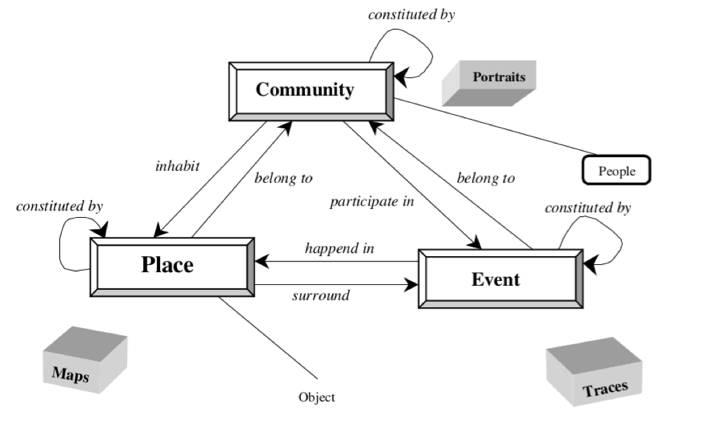
\includegraphics[scale=.5]{images/Figura2-1}
	\caption{\em Lógica de la 3-Ontology, extraído de Leiva-Lobos & Covarrubias (2002).}
	\label{fig:mt-im1}
\end{figure}

\begin{figure}
	\centering
	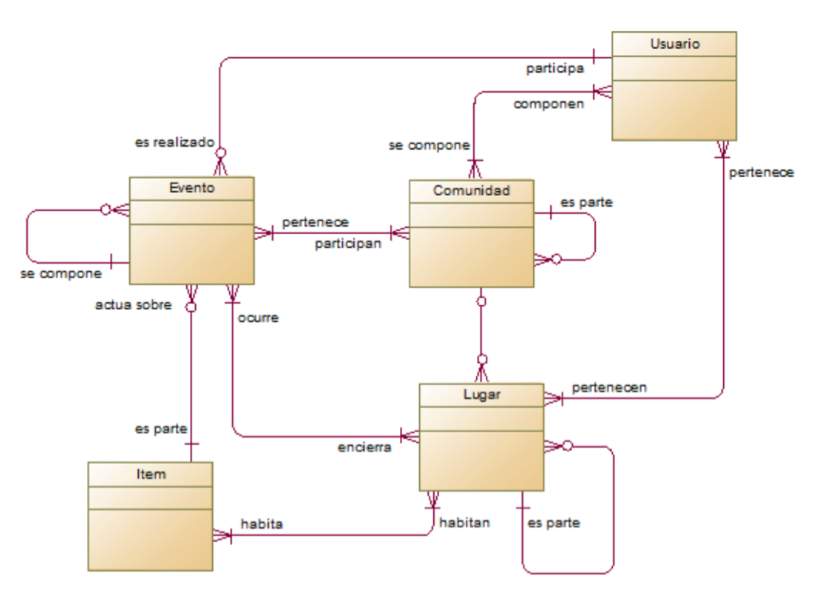
\includegraphics[scale=.5]{images/Figura2-2}
	\caption{\em Modelo conceptual de RBox, extraído de Vásquez (2013). }
	\label{fig:mt-im2}
\end{figure}

\section{Resumen}

En este capítulo se realizó una revisión de los fundamentos teóricos del trabajo de tesis. Para comenzar, se ha definido el concepto de red social. Luego, se presentó el concepto de análisis de redes sociales y los desafíos que supone para el área la inclusión de \textit{social media}. Posteriormente, se repasa el concepto de detección de comunidades y se explicitan distintas líneas de investigación. A continuación se trata el concepto de sistemas de recomendación de forma genérica y como han evolucionado a aquellos que consideran el contexto al momento de recomendar. Finalmente, se expone el concepto de la 3-Ontology, junto con los contenedores de sentido y se aborda una contribución de este trabajo de tesis a una implementación basada en este \textit{framework}.

%--------Visión General de la Solución
%--------Daniel Ochoa John
%--------05/06/2012

\chapter{Visión general de la solución}
\label{cap:vision}
En este capítulo se describe conceptualmente la solución desarrollada en este trabajo de tesis. En primer lugar, se expone el modelamiento que fundamenta el desarrollo de los distintos componentes de \textit{software} que este trabajo presenta. Posteriormente, se describe el mecanismo de \textit{community \textit{cache}} detonado al momento de recomendar. Luego, se explica cómo esos conceptos son transformados en un modelamiento de \textit{software}.  Finalmente, se muestra la integración entre los distintos componentes con apoyo de un diagrama general de la solución.

\section{Modelamiento}
\label{vision:redes}

En esta sección se detalla el modelamiento de los distintos aspectos involucrados en el desarrollo de este trabajo de tesis. El modelamiento sienta las bases sobre las que la solución es construída. En otras palabras, el resultado de este ejercicio conforma los requisitos funcionales que la solución debe contemplar. 

\subsection{Modelamiento de interacciones}

Como ya se ha mencionado anteriormente, en un contexto de social media pueden ocurrir diversas interacciones, como un mensaje, un ‘me gusta’, un follow, entre otras. En una red social hay diversas interacciones y depende del contexto y del dominio la relevancia de cada una de ellas en relación a su consideración en una recomendación hacia un usuario activo.

Son estas interacciones las que denotan a una comunidad. Por ejemplo, si en un contexto de una tienda virtual, un usuario realiza una valoración (\textit{rating}) mediante el método que fuere, como por ejemplo una valoración de un artículo en una escala del uno al cinco, dicha valoración será considerada, de una u otra manera, al momento de recomendar aquel artículo a otro usuario que pertenezca a la misma comunidad.

No obstante, diferentes interacciones pueden denotar muchos segmentos de interés para un usuario. Hipotéticamente hablando, si se considera un contexto de social media en el que sólo existen dos posibles interacciones: amistad y \textit{following}, es posible que un usuario establezca una interacción de amistad con personas que conozca físicamente o virtualmente. No obstante, es posible que genere eventos de \textit{following} con personas relacionadas con temas en boga, como una noticia importante, algún evento deportivo, entre otras. Ante esto pueden ocurrir dos situaciones principales, que los segmentos o comunidades de interés denotadas por ambas interacciones para un usuario sean similares, o que ambas interacciones determinen segmentos de interés divergentes entre sí.

En RBox, las interacciones son modeladas a través de eventos, siguiendo las directrices establecidas por el meta modelo de la 3-Ontology. Pragmáticamente, existe una interfaz llamada Event (ver Figura \ref{fig:vis-im1}), que define este meta modelo. Por lo que todo evento debe tener un valor y contextualmente debe ser realizado por un usuario, enfocado en un objeto en particular (que puede ser otro usuario), situado en una comunidad, realizado en un lugar en particular y debe contar con una marca temporal. 

\begin{figure}
  \centering
  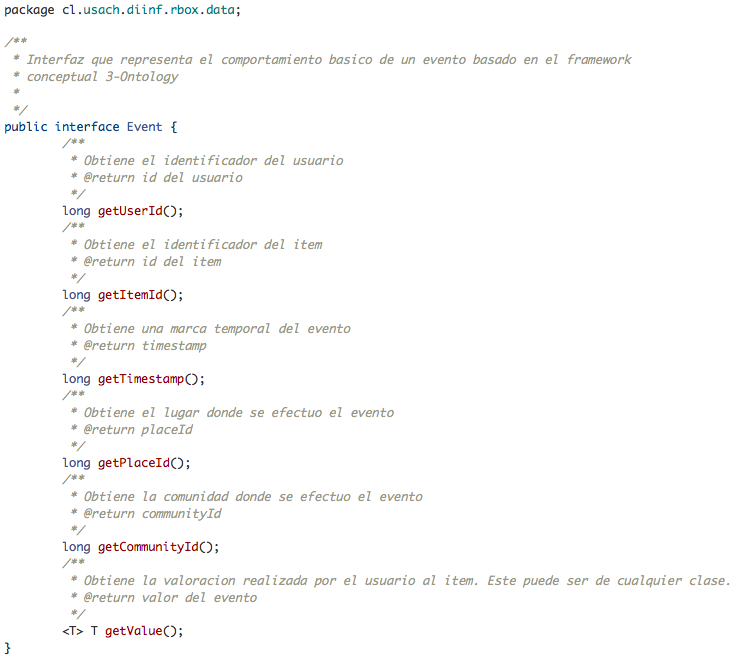
\includegraphics[scale=.5]{images/Figura7-1}
  \caption{\em Interfaz Event del código fuente de RBox.}
  \label{fig:vis-im1}
\end{figure}

Entonces, uno de los problemas que deben ser resueltos en la implementación de la solución es el de realizar una correspondencia entre el modelo de datos del dominio situado en un ambiente de social media y una definición de evento tipada por RBox.

\subsection{Modelamiento de la detección de comunidades}

En ese sentido y considerando lo anterior, es que la detección de comunidades que la solución provea debe considerar a aquellas que están latentes en el dominio de los distintos eventos. Por ende, es necesario abstraer el concepto de evento de manera tal que la solución sea capaz de detectar comunidades en base a todas aquellas interacciones que sean definidas como relevantes para un cierto dominio de análisis. 

En el mundo de la tecnología (y de los repositorios de código) existen distintas librerías que implementan mecanismos y técnicas para detectar comunidades que existen en la literatura:

\begin{itemize}
	\item Gephi (gephi.github.io/)
	\item igraph (igraph.org/)
	\item graph-tool (graph-tool.skewed.de/)
	\item JGraphT (jgrapht.org/)
	\item GraphStream (graphstream-project.org/)
	\item entre otras ... 
\end{itemize}

Su uso, en desmedro de implementar los algoritmos desde su publicación, tiene la tiene la gran ventaja de contar con una comunidad que respalda su uso, funcionamiento, resultados y que además hace el código mantenible.

No obstante, es claro notar que estas librerías, o APIs, están enfocadas en un modelamiento en base a grafos, en donde los nodos representan a los usuarios de una red social y las aristas representan una conexión (a partir de interacciones, según la red social) entre dos usuarios. Por ende, otro de los problemas que deben ser resueltos por la solución presentada por este trabajo, es el de encapsular la información contenida por las distintas instancias de los objetos que pertenezcan una clase que implemente la interfaz Event, con el objetivo de generar un grafo de interacciones.

Al contar con un grafo de interacciones, es posible utilizar las APIs disponibles para análisis de grafos (la detección de comunidades incluida) con el objetivo de detectar las comunidades latentes, que existen en aquel grafo.

\subsection{La 3-Ontology y las comunidades}

Las comunidades son una dimensión considerada en el meta modelo de la 3-Ontology y está definida en el \textit{framework} de RBox como muestra el código de la Figura \ref{fig:vis-im2}. Una comunidad, entonces, está formada principalmente por un conjunto de usuarios. Cuando se hace uso de la detección de comunidades, se debe contar con un mecanismo o componente que sea capaz de integrar los dos mundos: el de la teoría de grafos con el correspondiente a la 3-Ontology.

\begin{figure}
  \centering
  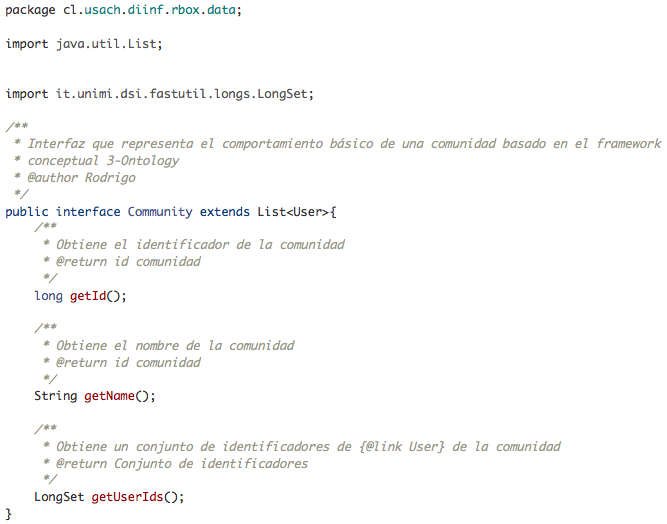
\includegraphics[scale=.5]{images/Figura7-2}
  \caption{\em Interfaz Community del código fuente de RBox.}
  \label{fig:vis-im2}
\end{figure}

Como se ha mencionado en la sección anterior, el componente que sea responsable de manejar la detección de comunidades, estará trabajando bajo un dominio de la teoría de grafos y no necesariamente debe inmiscuirse con el meta modelo planteado por la 3-Ontology. Esto fundamentado en el principio de única responsabilidad (single responsibility principle, en inglés) en la ingeniería de \textit{software} (Martin, 2003), el cual plantea que cada componente de una aplicación debe responder a un propósito atómico e independiente. En ese sentido, la detección de comunidades puede ser considerado un propósito independiente del proceso o \textit{framework} que haga uso de sus beneficios. 
    
Lo anterior genera una arista adicional a considerar en el diseño de la solución que es, precisamente, la integración entre los dos mundos. Debe existir un componente, herramienta o librería que sea capaz de realizar una transformación desde la meta información que contiene un grafo con comunidades detectadas, hasta un esquema definido en base a las directrices que plantea la 3-Ontology, es decir, pasar de un conjunto de nodos y aristas pertenecientes a un \textit{‘cluster’}, hacia una comunidad, que contiene un conjunto de usuarios.

\section{Community Cache}

El objetivo principal de este trabajo es verificar si contar con un mecanismo de \textit{‘\textit{cache}’} para manejar las comunidades en ejecuciones previas de un sistema de recomendación, permite mejorar el tiempo de respuesta que es requerido para otorgar una recomendación a un usuario activo. En ese contexto, es necesario definir el mecanismo de \textit{cache} que será construído y como actúa en el flujo actual de la recomendación, planteado por el \textit{framework} RBox.

Este flujo considera (de izquierda a derecha en la Figura \ref{fig:vis-im3}) , precisamente, un \textit{mapping} desde una red social hacia la lógica de la 3-Ontology. Posteriormente, para un usuario activo se tiene definición de los contenedores de sentido: comunidades, eventos y lugares. Luego, y al momento de realizar una recomendación, se toma en cuenta aquellos contenedores de sentido tipificados por distintos factores, como el contexto temporal en el que fueron realizados, como por ejemplo, lugares visitados entre una fecha y otra.

\begin{figure}
  \centering
  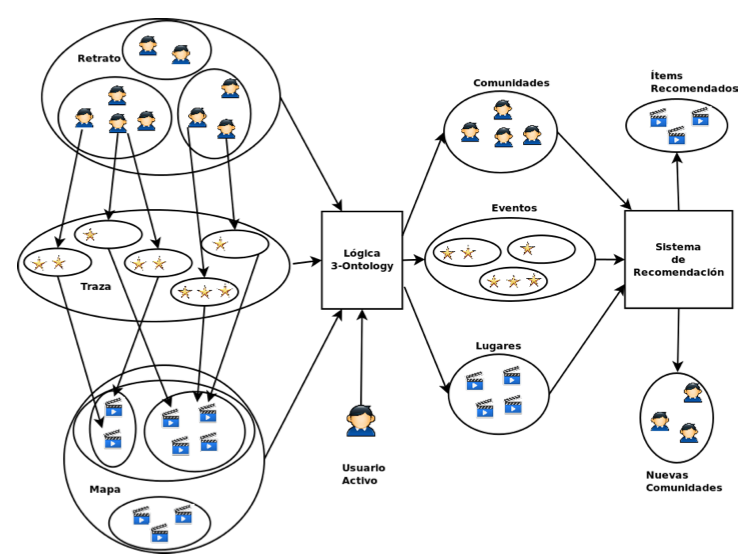
\includegraphics[scale=.5]{images/Figura7-3}
  \caption{\em Flujo propuesto por RBox para llevar a cabo una recomendación.}
  \label{fig:vis-im3}
\end{figure}

Lo anterior da como resultado un conjunto de ítems recomendados, así como también nuevas comunidades. Son estas comunidades las que deben ser persistidas y, de esta manera, estar disponibles para su uso como retroalimentación hacia recomendaciones posteriores. Una \textit{cache} es necesaria debido a que cabe la posibilidad de que las comunidades detectadas en distintas iteraciones del algoritmo de recomendación ya hayan sido detectadas en iteraciones precedentes, por lo que su manejo debe ser tratado con mayor ligereza que aquellas que son detectadas por primera vez. El concepto de ligereza en el manejo de las comunidades pasa por incorporar al mecanismo de \textit{cache} dos niveles de manejo: uno que faculte la activación o no de la detección de comunidades en una recomendación y otro que maneje, de cierta forma, las distintas apariciones de las comunidades detectadas.

\subsection{Primer nivel de \textit{cache}}

El primer nivel de \textit{cache} considera un mecanismo para enfrentar el escenario en el cual no existen comunidades detectadas para un usuario. Si el contexto de social media en el que un recomendador esté funcionando no considera de manera explícita el concepto de comunidad (por ejemplo, Google+ si lo hace), entonces en el esquema de la 3-Ontology, los usuarios no tendrían comunidades asociadas en primera instancia.

No obstante, lo anterior no quiere decir que estas no existan, por lo que se define un mecanismo que active la detección de comunidades si un usuario activo no pertenece a ninguna comunidad. En el caso de redes sociales de \textit{microblogging}, como Twitter, las comunidades no son explícitas y la gran cantidad de tópicos que son tratados (y a la velocidad que son tratados), implica que un usuario puede estar inmerso en distintas comunidades, de manera implícita.

Esto puede tener un impacto en el tiempo requerido para realizar una recomendación. Ciertamente, el proceso de detección de comunidades durante la generación de una recomendación, representa un costo de tiempo adicional. A esto hay que agregar el tiempo requerido para operaciones de persistencia, como lectura y escritura de una base de datos, por ejemplo.

Luego, el primer nivel de \textit{cache} permite establecer una estrategia de detección de comunidades, en la que, por ejemplo, se puede utilizar un proceso que, luego de cierto tiempo planificado, desactive el primer nivel de \textit{cache}, con la finalidad de actualizar las comunidades a las que pertenece un usuario. Esto en desmedro de realizar la detección de comunidades de manera recurrente y cada vez que una aplicación lo requiera.

\subsection{Segundo nivel de \textit{cache}}

El segundo nivel de \textit{cache} es un mecanismo de manejo de las comunidades ya detectadas. Lo que se busca es mitigar, de cierta forma, el aumento en el tiempo necesario para realizar una recomendación considerando detección de comunidades. Si se asume que una comunidad puede ser detectada más de una vez, en más de una iteración del algoritmo de recomendación, entonces lo que se debe hacer es identificar que esa comunidad ya existe.

Cuando una comunidad ya ha sido detectada en iteraciones anteriores del algoritmo, no deben ocurrir las operaciones de persistencia. Se debe evaluar si una comunidad detectada (C’) existe en el medio persistente (C) comparando al conjunto de usuarios (u) que éstas contienen.  Si ambos conjuntos, digamos Cu y C’u son iguales, entonces las comunidades son iguales (\textit{hit}) y la persistencia de la comunidad detectada debe omitirse. En caso contrario (\textit{miss}), las operaciones de persistencia para la comunidad detectada deben ejecutarse.

Lo que se pretende es provocar un efecto de reducción de tiempo al mediano plazo. Lógicamente, en las primeras iteraciones del algoritmo, la cantidad de \textit{hits} será menor a la cantidad de \textit{miss} al momento de evaluar la persistencia de una comunidad detectada. No obstante, a medida que las recomendaciones ocurran, es posible que el proceso de detección de comunidades arroje resultados que ya han ocurrido en iteraciones anteriores, por lo que el mecanismo de persistencia para esa comunidad no será efectuado. Luego, se ahorra el tiempo requerido para ello y la recomendación ocurrirá más rápido.

\section{Componentes de \textit{software}}

En las secciones anteriores se realizó un análisis de aquellas dificultades y consideraciones que debe tener la solución. En esta sección se analizarán las características y responsabilidades que deben tener los componentes de \textit{software}, que serán desarrollados con la finalidad de superar aquellas dificultades y manejar aquellas consideraciones.

\subsection{Manejo de las interacciones}

En primer lugar, deben manejarse adecuadamente las interacciones que existen en un ambiente de social media, con el fin de abordar el problema de correspondencia entre el modelo de datos del dominio y la definición de evento tipada por RBox. En ese sentido, debe existir un componente de \textit{software} que permite realizar un mapeo entre estos dos dominios y exportar hacia un medio persistente la información de las interacciones realizadas por los usuarios.

Este componente debe conectarse al ambiente de social media a través del método más “limpio” posible. Es decir, si el ambiente cuenta con una API disponible para acceder a su información, este método debe ser preferido por sobre otros, como por ejemplo adoptar una estrategia de scrapping.

La estrategia de extracción debe considerar la mayor cantidad de información que las políticas de privacidad de los ambientes permitan y debe tender a completar lo más posible el modelamiento de datos utilizado por RBox, y que está basado en el marco otorgado por la 3-Ontology.

Por otro lado, se deben definir las interacciones del dominio de extracción en RBox. Esto pasa por identificar, tipificar y crear una jerarquía de clases de manera tal que cada una de las interacciones que ocurren en un dominio determinado, deben corresponder, en RBox, a una clase que herede de Evento.

\subsection{Detección de comunidades}

En segundo lugar, debe existir un componente de \textit{software} que otorgue funcionalidad de detección de comunidades. Este componente debe ser construído de manera tal que su integración con RBox no sea invasiva, permitiendo su reemplazo por otros componentes similares, según se requiera.

Como parte de la integración, debe ser abordado el problema de encapsulación de los distintos eventos definidos en RBox, con el objetivo de generar un grafo de interacciones. Este grafo de interacciones debe ser genérico y no debe importar el evento que propicie su construcción. Luego, el componente de \textit{software} debe ser capaz de interpretar este grafo de interacciones y debe proveer diversos mecanismos para realizar detección de comunidades. La respuesta de este componente debe ser un grafo con sus comunidades explicitadas.

\subsection{Persistencia de comunidades}

En tercer lugar, debe existir un componente de \textit{software} que maneje la persistencia de las comunidades detectadas. Entre las responsabilidades de este componente está la de conectarse con el componente de detección de comunidades, incorporando a RBox un servicio que faculte a todo sistema de recomendación desarrollado con el \textit{framework}, el uso de la detección de comunidades.

Uno de los principales desafíos que aborda este componente es el de implementar el mecanismo de \textit{community \textit{cache}} descrito en la sección anterior. Este mecanismo se debe detonar cuando comiencen las operaciones que tengan relación con la persistencia de las comunidades.

La persistencia ocurre al momento de interpretar y transformar desde el grafo con comunidades explicitadas, que es salida del componente de detección de comunidades, hacia el modelo de comunidades que maneja RBox. Es en este momento cuando deben añadirse operaciones al DAO de RBox para que sea capaz de detectar comunidades con un conjunto de usuarios idénticos.

Además, este componente debe integrarse a RBox implementando todos aquellos servicios de DAO que tengan relación con el manejo de las comunidades y que en su primera versión se han dejado sin implementar. Esto con el objetivo de completar el conjunto de herramientas que el API de RBox provee a los desarrolladores de sistemas de recomendación.

\section{Integración de componentes}

Los componentes descritos anteriormente deben integrarse de diversas maneras. La Figura \ref{fig:vis-im4} muestra un diagrama que representa conceptualmente esta integración, entre paréntesis están descritos los nombres de referencia que aparecen en la Figura. En primer lugar está el componente (\textit{\textit{mapping} component}), que resuelve la extracción de interacciones y sus transformaciones a eventos.

\begin{figure}
  \centering
  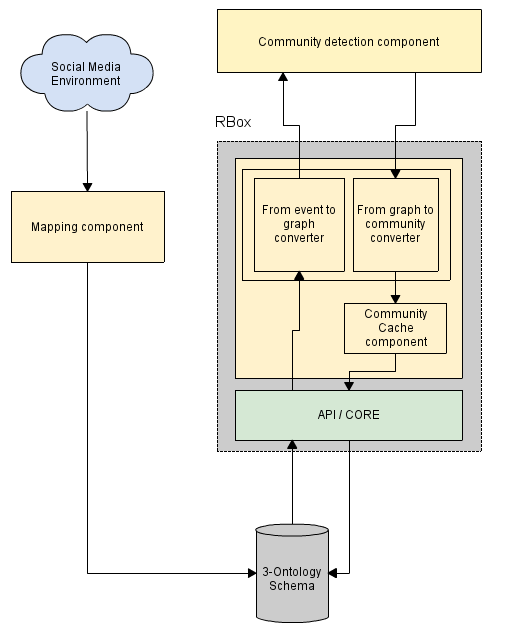
\includegraphics[scale=.5]{images/Figura7-4}
  \caption{\em Diagrama conceptual de integración de los componentes de \textit{software}.}
  \label{fig:vis-im4}
\end{figure}

Este componente extrae información desde el ambiente de social media (\textit{social media environment}) a través del mecanismo más limpio como ya se mencionó anteriormente y persiste estas interacciones en un medio persistente, cuyo esquema está en regla con el definido por la 3-Ontology (3-Ontology \textit{Schema}).

Con el medio persistente ya con eventos, y suponiendo que se está en proceso de recomendación, el componente que convierte los eventos a grafos (\textit{From event to graph converter}), a través de las operaciones de DAO definidas en el API y el CORE de RBox, extrae aquellos eventos que sean de interés y construye un grafo de interacciones.

Posteriormente, este grafo de interacciones es enviado al componente de detección de comunidades (\textit{Community detection component}), que interpreta el grafo, lo procesa y detecta las comunidades mediante un método que le es definido.

Este último componente retorna la información del grafo con comunidades hacia un componente de transformación de grafos a comunidades (\textit{From graph to community converter}) que interpreta este grafo en el esquema definido por la 3-Ontology para las comunidades.

Luego, se procede a las operaciones de persistencia de las comunidades detectadas, por lo que se da inicio a la intervención del componente que maneja la \textit{community \textit{cache}}, quién filtra las comunidades ya persistidas. Esto permite que, luego y nuevamente por operaciones del DAO, se persistan aquellas comunidades detectadas en la ejecución actual del algoritmo de recomendación. Finalmente, se prosigue con la ejecución del algoritmo con normalidad.

\section{Resumen}

En este capítulo se han abordado los desafíos y problemáticas derivadas del cumplimiento del objetivo general de este trabajo de tesis. Se  han descrito aquellos componentes que deben ser incorporados a RBox con la finalidad de proveer una plataforma tecnológica que permite probar la hipótesis propuesta. En los capítulos siguientes se describe con mayor detalle a los componentes de \textit{software} diseñados en este capítulo, con sus implementaciones concretas, arquitecturas y paradigmas utilizados.
























%--------Sericio para la detección de comunidades
%--------Daniel Ochoa John
%--------20/07/2014
\newcolumntype{L}[1]{>{\raggedright\let\newline\\\arraybackslash\hspace{0pt}}m{#1}}
\newcolumntype{C}[1]{>{\centering\let\newline\\\arraybackslash\hspace{0pt}}m{#1}}
\newcolumntype{R}[1]{>{\raggedleft\let\newline\\\arraybackslash\hspace{0pt}}m{#1}}


\chapter{Servicio para la detección de comunidades}
\label{cap:servicio}

En este capítulo se describe el servicio de detección de comunidades que se desarrolló en este trabajo de tesis. En primer lugar, se caracteriza y describe a la arquitectura y sus componentes. Posteriormente, se declaran los algoritmos y \textit{endpoints} utilizados por el servicio. Finalmente, se muestra un ejemplo de funcionamiento con un problema clásico de la literatura.

\section{Caracterización del Servicio}

En la presente sección, se realiza una caracterización del servicio que se ha construido, desde un punto de vista, tanto tecnológico, en relación a aquellas herramientas desarrolladas para responsabilidades funcionales específicas e ingenieril, en relación a la combinación y comunicación de aquellas herramientas, para alcanzar un objetivo mayor.

\subsection{Descripción general}

Una de las principales dificultades de este trabajo de tesis ha sido la de añadir a RBox la capacidad de detectar comunidades de una manera limpia, es decir, sin afectar el funcionamiento actual del sistema. Esto implica que dicha añadidura no debe suponer, por una parte, una mayor reingeniería de los componentes que ya se han definido en la herramienta y por otra, una estricta dependencia de RBox con respecto al componente de detección de comunidades. En resumen, la nueva pieza de \textit{software} que se ha incorporado debe cumplir con los siguientes requisitos:

\begin{enumerate}[I]
  \item{No debe implicar modificaciones en el código de los componentes ya definidos.}
  \item{La pieza debe ser capaz de detectar comunidades.}
  \item{La pieza no debe impedir su reemplazo por otra con mayores prestaciones o mucho más específica.}
\end{enumerate}

Siguiendo estos tres principios básicos definidos para la aplicación, es que se ha tomado como alternativa una arquitectura orientada a servicios, ya que permite flexibilidad al integrarse con sistemas “legados” (Bianco, Kotermanski, & Merson, 2007).  Continuando con la misma línea de pensamiento, al momento de definir que tipo de servicio conviene disponibilizar, si un servicio Web SOAP\footnote{SOAP es el acrónimo de \textit{Simple Object Access Protocol}, que define un \textit{stack} de componentes para el intercambio de información entre aplicaciones.} convencional o un servicio de tipo REST\footnote{REST es el acrónimo de \textit{Representaton State Transfer}, que engloba y define una manera de acceder a recursos a través de la web únicamente utilizando el protocolo HTTP.}, se ha probado y evidenciado que los servicios de tipo REST son mayormente adecuados cuando se requieren integraciones estratégicas con otras aplicaciones, cuando el performance importa (Guinard, Ion, & Mayer, 2012). Luego, el servicio construido es de tipo REST.

Ahora bien, de las alternativas posibles para proveer un servicio que sea eficaz detectando comunidades: construir una librería con distintos algoritmos o seleccionar y adaptar una existente, se ha optado por la segunda alternativa, ya que existe una librería llamada igraph (Csárdi & Nepusz, 2006), construída bajo C, que provee diferentes estrategias y algoritmos típicamente utilizados para el análisis de grafos y en específico, la detección de comunidades. Esta librería cuenta con un encapsulamiento de la implementación en C hacia Python, lo que permite comunicar sus prestaciones con un \textit{framework} que soporte la construcción de servicios Web de tipo REST.

\subsection{Arquitectura del Servicio}

Como primer antecedente, y para contextualizar, es necesario mencionar la arquitectura que se ha definido para la construcción del servicio. La Figura \ref{fig:serv-im1} muestra un diagrama con los componentes definidos y sus interacciones. La descripción de cada uno de ellos es la siguiente:

\begin{itemize}
  \item \textbf{\textit{Client}:} es una aplicación, servicio o componente de \textit{software} que requiere un servicio de análisis de comunidades y, en concreto, un servicio de detección de comunidades. Este cliente debe preocuparse de encapsular la información de manera conveniente a la que el servicio espera al momento de realizar la petición de servicio, así como también de traducir la respuesta del recién mencionado. En el diagrama, esta situación se refleja como \textit{Wrapped Data}.
  \item \textbf{\textit{Network Environment}:} representa al ambiente de red que separa al cliente y al servicio. Es muy relevante considerarlo debido a que, dependiendo del tamaño del problema, es posible que el ambiente del cliente no requiera uno de alta disponibilidad de recursos (a.k.a \textit{cloud servers}). Sin embargo, el servicio puede abastecer a muchísimos clientes, por lo que puede requerir un ambiente escalable horizontalmente para su \textit{deployment}, como por ejemplo la nube de \textit{Amazon}.
  \item \textbf{Endpoints:} son las interfaces que expone el servicio para que los clientes se comunican con él. En el caso del servicio de detección de comunidades, cada \textit{endpoint} implica un algoritmo diferente para realizar la detección de comunidades.
  \item \textbf{Servicio:} el servicio es el resultado de la unión de distintas tecnologías. En primer lugar, y para permitir la exposición de un servicio Web de tipo rest, se utiliza flask-restful\footnote{Sitio web oficial en http://flask-restful.readthedocs.org/en/latest}. Luego, para permitir la comunicación con igraph, se utiliza un componente que encapsula la comunicación con la mencionada librería, llamada python-igraph. Finalmente, para todo el procesamiento y disponibilización de algoritmos, se utiliza la librería igraph. La especificación tanto de python-igraph como de igraph está disponible en el sitio Web oficial\footnote{Sitio web oficial de igraph para python en http://igraph.org/python/.}.
\end{itemize}

\begin{figure}
  \centering
  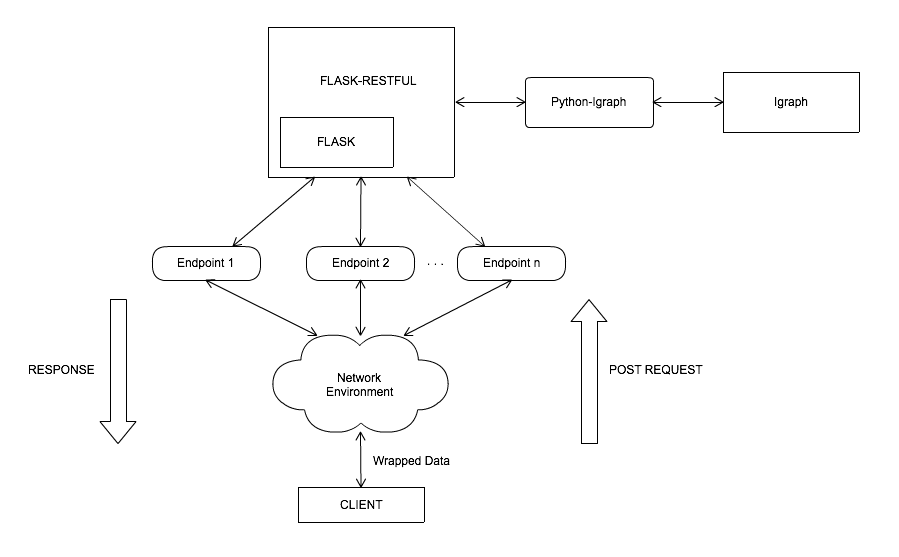
\includegraphics[scale=.5]{images/Figura3-1}
  \caption{\em Arquitectura del servicio de detección de comunidades.}
  \label{fig:serv-im1}
\end{figure}

\section{Algoritmos Utilizados}

En esta sección se enuncian los algoritmos que se han publicado mediante el servicio de detección de comunidades y que son aquellos que la librería igraph ha implementado. La Tabla \ref{tab:serv-tab01} muestra a cada uno de ellos y el endpoint en particular al que están sujetos.

\begin{enumerate}[I]
  \item \textbf{Multilevel} (Blondel, Guillaume, Lambiotte, \& Lefebvre, 2008): Maximización de la modularidad en donde los vecinos se juntan en comunidades, los cuales se juntan en comunidades de comunidades. En primer lugar, cada nodo se asigna a su propio módulo y luego cada nodo se mueve al módulo vecino que produzca el mayor aumento a la modularidad. Si no ocurre aumento alguno con ningún movimiento, entonces el nodo permanece en su módulo. Cada nodo puede ser considerado más de una vez. La red se reconstruye considerando a los módulos como nuevos nodos y se aplica el algoritmo nuevamente. Esto se repite hasta que la modularidad no puede ser maximizada.
  \item \textbf{Label Propagation} (Raghavan, Albert, \& Kumara, 2007): A cada uno de los nodos de un grafo se le asigna una marca o label. El procedimiento continúa iterativamente y a cada nodo se le asigna la marca mas frecuente de sus vecinos de una manera síncrona. El método se detiene cuando la marca de cada nodo es una de las marcas más frecuentes en su cluster o barrio. Es muy rápido, no obstante es no determinista.
  \item \textbf{Leading Eigenvector} (Newman, 2006): Enfoque jerárquico que optimiza la función de la modularidad. En cada iteración, el grafo se divide en dos partes de manera que se produzca un aumento en la modularidad. La separación está determinada mediante un vector principal de modularidad (eigenvector) y existe una condición de término que impide que los grupos que están densamente conectados se separen.
  \item \textbf{Infomap} (Rosvall \& Bergstrom, 2008): Minimización de una ecuación que describe la cantidad de movimientos de un camino aleatorio en una red jerárquica. Sigue la filosofía del método de Louvain: los vecinos se juntan en módulos, los cuales se juntan en super-módulos. Cada nodo se asigna a su propio módulo y luego, de manera aleatoria, cada nodo se mueve al módulo vecino que produzca la mayor reducción de la ecuación. Si no ocurre reducción alguna con ningún movimiento, entonces el nodo permanece en su módulo. Ahora, la red se reconstruye considerando a los módulos como nuevos nodos y se aplica el algoritmo nuevamente. Hasta que la ecuación ya no pueda ser minimizada.
  \item \textbf{Spinglass} (Traag \& Bruggeman, 2009): Enfoque desde la física estadística. En este modelo cada nodo es considerado una partícula y puede estar en uno de los estados de spin. Las interacciones entre las partículas, las aristas, especifican quienes prefieren tener el mismo estado de spin y quienes prefieren cambiarlo. El modelo se simula para un número definido de iteraciones y el spin de las partículas determina quienes son una comunidad. Este método es no determinista.
\end{enumerate}

\begin{table}
  \begin{center}
    \caption[Estrategias utilizadas para la detección de comunidades.]{Estrategias utilizadas para la detección de comunidades.}
    \label{tab:serv-tab01}
      \begin{tabular}{|L{6cm}|L{5cm}|}
        \hline
        \textbf{Algoritmo} & \textbf{Endpoint (POST)}\\ \hline
         \textit{Multilevel} &  /CommunityDetection/Multilevel \\ \hline
         \textit{Label Propagation} & /CommunityDetection/LabelPropagation \\ \hline
         Leading Eigenvector & /CommunityDetection/LeadingEigenvector \\ \hline
         Infomap  & /CommunityDetection/Infomap \\ \hline
         Spinglass & /CommunityDetection/Spinglass \\ \hline
      \end{tabular}
  \end{center}
\end{table}

\section{Ejemplo de Funcionamiento}

En esta sección se muestra el funcionamiento del servicio de detección de comunidades a partir de un ejemplo clásico en la literatura, que es detectar las comunidades en el club de karate de Zachary (Zachary, 1977), que tiene 34 nodos, 78 aristas y el máximo componente conectado es de 34 nodos. Para esto, se han destinado endpoints (ver Tabla \ref{tab:serv-tab02})  del servicio de manera tal que el ejemplo sea parte de la aplicación:

\begin{table}[H]
  \begin{center}
    \caption[Servicios que implementan el manejo de la detección de comunidades en el Club de Karate de Zachary.]{Servicios que implementan el manejo de la detección de comunidades en el Club de Karate de Zachary.}
    \label{tab:serv-tab02}
      \begin{tabular}{|L{6cm}|L{10cm}|}
        \hline
        \textbf{Descripción} & \textbf{Endpoint (GET)}\\ \hline
         JSON que representa el grafo del problema del club de karate de Zachary. & /KarateClub \\ \hline
         JSON que representa a las comunidades detectadas en el \textit{data\textit{set}} del club de karate de Zachary utilizando el mismo algoritmo que el \textit{endpoint} /CommunityDetection/\textit{Multilevel}. & /KarateClub/Communities/\textit{Multilevel} \\ \hline
         JSON que representa a las comunidades detectadas en el \textit{data\textit{set}} del club de karate de Zachary utilizando el mismo algoritmo que el \textit{endpoint} /CommunityDetection/LabelPropagation & /KarateClub/Communities/LabelPropagation \\ \hline
         JSON que representa a las comunidades detectadas en el \textit{data\textit{set}} del club de karate de Zachary utilizando el mismo algoritmo que el \textit{endpoint} /CommunityDetection/LeadingEigenvector & /KarateClub/Communities/LeadingEigenvector \\ \hline
         JSON que representa a las comunidades detectadas en el \textit{data\textit{set}} del club de karate de Zachary utilizando el mismo algoritmo que el \textit{endpoint} /CommunityDetection/Infomap & /KarateClub/Communities/Infomap \\ \hline
         JSON que representa a las comunidades detectadas en el \textit{data\textit{set}} del club de karate de Zachary utilizando el mismo algoritmo que el \textit{endpoint} /CommunityDetection/Spinglass & /KarateClub/Communities/Spinglass \\ \hline
      \end{tabular}
  \end{center}
\end{table}

La Figura \ref{fig:serv-im2} muestra el grafo que se genera al realizar el \textit{parsing} correspondiente luego de hacer el \textit{request} a /KarateClub. Cuando se realiza el \textit{request} a /KarateClub/Communities para detectar las comunidades que existen en el \textit{data\textit{set}} de Zachary el resultado, para cada algoritmo, se muestra desde la Figura \ref{fig:serv-im3} hasta la Figura \ref{fig:serv-im7}. La Tablas \ref{tab:serv-tab03} a \ref{tab:serv-tab07} describen las comunidades detectadas por extensión, para cada algoritmo:

\begin{figure}
  \centering
  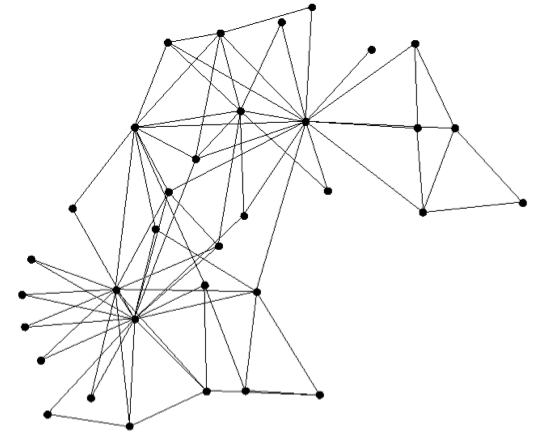
\includegraphics[scale=.6]{images/Figura3-2}
  \caption{\em Grafo que representa al Club de Karate de Zachary.}
  \label{fig:serv-im2}
\end{figure}

\begin{figure}[H]
  \centering
  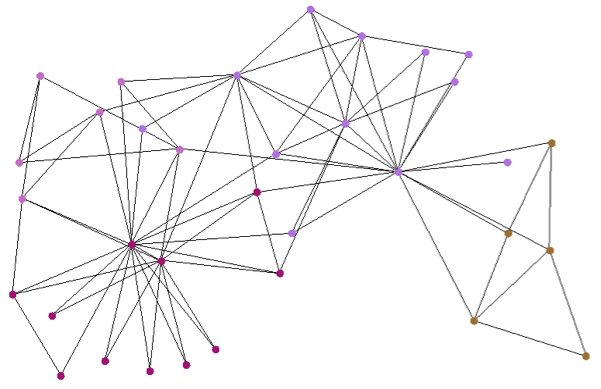
\includegraphics[scale=.6]{images/Figura3-3}
  \caption{\em Comunidades detectadas en el Club de Karate mediante el método \textit{\textit{Multilevel}}.}
  \label{fig:serv-im3}
\end{figure}

\begin{table}[H]
  \begin{center}
    \caption{Definición por extensión de las comunidades detectadas en el Club de Karate mediante el método \textit{\textit{Multilevel}}.}
    \label{tab:serv-tab03}
      \begin{tabular}{|L{4cm}|L{10cm}|}
        \hline
        \textbf{Nº Comunidad} & \textbf{Nodos}\\ \hline
         1 & 5, 6, 7, 11, 17 \\ \hline
         2 & 1, 2, 3, 4, 8, 10, 12, 13, 14, 18, 20, 22 \\ \hline
         3 & 24, 25, 26, 28, 29, 32 \\ \hline
         4 & 9, 15, 16, 19, 21, 23, 27, 30, 31, 33, 34 \\ \hline
      \end{tabular}
  \end{center}
\end{table}

\begin{figure}[H]
  \centering
  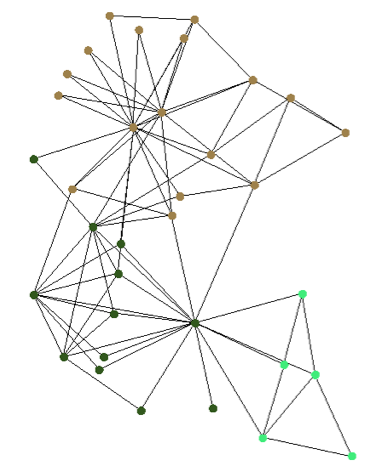
\includegraphics[scale=.6]{images/Figura3-4}
  \caption{\em Comunidades detectadas en el Club de Karate mediante una ejecución del método \textit{Label Propagation}.}
  \label{fig:serv-im4}
\end{figure}

\begin{table}[H]
  \begin{center}
    \caption{Definición por extensión de las comunidades detectadas en el Club de Karate mediante una ejecución del método \textit{Label Propagation}.}
    \label{tab:serv-tab04}
      \begin{tabular}{|L{4cm}|L{10cm}|}
        \hline
        \textbf{Nº Comunidad} & \textbf{Nodos}\\ \hline
         1 & 1, 2, 3, 4, 8, 10, 12, 13, 14, 18, 20, 22 \\ \hline
         2 & 5, 6, 7, 11, 17 \\ \hline
         3 & 9, 15, 16, 19, 21, 23, 24, 25, 26, 27, 28, 29, 30, 31, 32, 33, 34 \\ \hline
      \end{tabular}
  \end{center}
\end{table}

\begin{figure}[H]
  \centering
  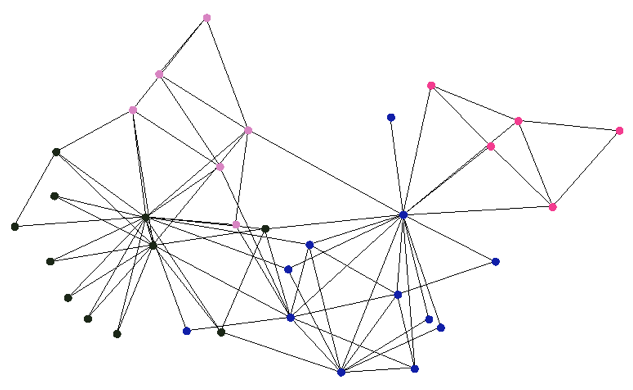
\includegraphics[scale=.6]{images/Figura3-5}
  \caption{\em Comunidades detectadas en el Club de Karate mediante el método \textit{Spinglass}.}
  \label{fig:serv-im5}
\end{figure}

\begin{table}[H]
  \begin{center}
    \caption{Definición por extensión de las comunidades detectadas en el Club de Karate mediante el método \textit{Spinglass}.}
    \label{tab:serv-tab05}
      \begin{tabular}{|L{4cm}|L{10cm}|}
        \hline
        \textbf{Nº Comunidad} & \textbf{Nodos}\\ \hline
         1 & 24, 25, 26, 28, 29, 32 \\ \hline
         2 & 5, 6, 7, 11, 17 \\ \hline
         3 & 1, 2, 3, 4, 8, 10, 12, 13, 14, 18, 20, 22 \\ \hline
         4 & 9, 15, 16, 19, 21, 23, 27, 30, 31, 33, 34 \\ \hline
      \end{tabular}
  \end{center}
\end{table}

\begin{figure}[H]
  \centering
  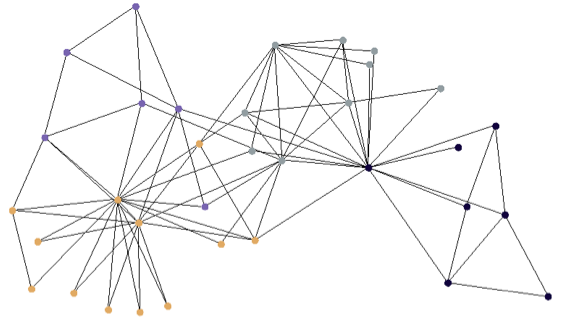
\includegraphics[scale=.6]{images/Figura3-6}
  \caption{\em Comunidades detectadas en el Club de Karate mediante el método \textit{LeadingEigenvector}.}
  \label{fig:serv-im6}
\end{figure}

\begin{table}[H]
  \begin{center}
    \caption{Definición por extensión de las comunidades detectadas en el Club de Karate mediante el método \textit{LeadingEigenvector}.}
    \label{tab:serv-tab06}
      \begin{tabular}{|L{4cm}|L{10cm}|}
        \hline
        \textbf{Nº Comunidad} & \textbf{Nodos}\\ \hline
         1 & 1, 5, 6, 7, 11, 12, 17 \\ \hline
         2 & 9, 10, 15, 16, 19, 21, 23, 27, 30, 31, 33, 34 \\ \hline
         3 & 2, 3, 4, 8, 13, 14, 18, 20, 22 \\ \hline
         4 & 24, 25, 26, 28, 29, 32 \\ \hline
      \end{tabular}
  \end{center}
\end{table}

\begin{figure}[H]
  \centering
  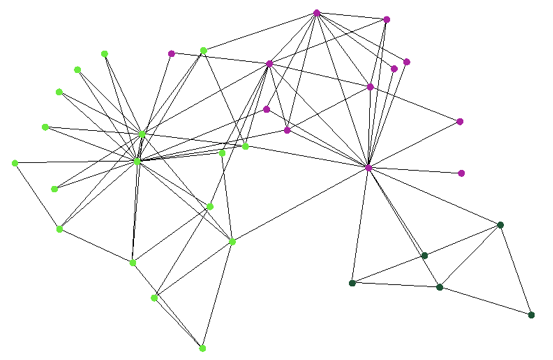
\includegraphics[scale=.6]{images/Figura3-7}
  \caption{\em Comunidades detectadas en el Club de Karate mediante el método \textit{Infomap}.}
  \label{fig:serv-im7}
\end{figure}

\begin{table}[H]
  \begin{center}
    \caption{Definición por extensión de las comunidades detectadas en el Club de Karate mediante el método \textit{Infomap}.}
    \label{tab:serv-tab07}
      \begin{tabular}{|L{4cm}|L{10cm}|}
        \hline
        \textbf{Nº Comunidad} & \textbf{Nodos}\\ \hline
         1 & 1, 2, 3, 4, 8, 10, 12, 13, 14, 18, 20, 22 \\ \hline
         2 & 5, 6, 7, 11, 17 \\ \hline
         3 & 9, 15, 16, 19, 21, 23, 24, 25, 26, 27, 28, 29, 30, 31, 32, 33, 34 \\ \hline
      \end{tabular}
  \end{center}
\end{table}

\section{Resumen}

En este capítulo se presentó el servicio de detección de comunidades que se utilizará RBox. Se han descrito los fundamentos mediante los cuales se tomó la decisión de seleccionar tecnologías y componentes. Posteriormente, se ha descrito la arquitectura del servicio componente a componente. Finalmente, se han enunciado los \textit{endpoints} que proveerá el servicio y, mediante un ejemplo, se ha mostrado su funcionamiento detectando comunidades para un mismo \textit{data\textit{set}} y con distintos algoritmos.

%--------Arquitectura y Diseño de componente para RBox
%--------Daniel Ochoa John
%--------20/07/2014
\newcolumntype{L}[1]{>{\raggedright\let\newline\\\arraybackslash\hspace{0pt}}m{#1}}
\newcolumntype{C}[1]{>{\centering\let\newline\\\arraybackslash\hspace{0pt}}m{#1}}
\newcolumntype{R}[1]{>{\raggedleft\let\newline\\\arraybackslash\hspace{0pt}}m{#1}}

\chapter{Arquitectura y Diseño de componente para RBox}
\label{cap:arquitectura}

En este capítulo se tratará la arquitectura y diseño de un componente para RBox que permitirá comunicarse apropiadamente con el componente de detección de comunidades ya descrito en el Capítulo 3. En primer lugar, se realizará una descripción de la arquitectura del componente, incluyendo su inclusión en RBox. Luego, se mostrará el diseño de clases con los componentes que ha sido necesario construir y se describen las razones de inclusión de cada uno de ellos. Posteriormente, se tratan los impactos que este componente ha tenido sobre las distintas capas de  RBox. Finalmente, se detalla la comunicación entre componentes y como se detona la detección de comunidades al recomendar.

\section{Descripción Arquitectural}

En esta sección se describe, en líneas generales, la arquitectura de RBox y su integración con las nuevas piezas de \textit{software} que permitirán consumir el servicio de detección de comunidades descrito anteriormente. La Figura \ref{fig:arq-im1} muestra los componentes utilizados y sobre los cuáles se ha diseñado.

\begin{figure}
  \centering
  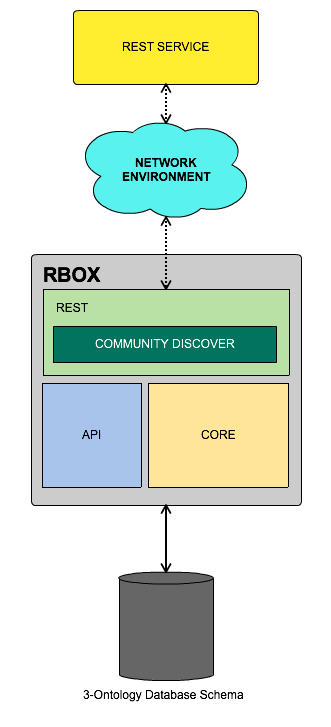
\includegraphics[scale=.6]{images/Figura4-1}
  \caption{\em Diagrama que representa la arquitectura formada por los componentes de RBox.}
  \label{fig:arq-im1}
\end{figure}


En primer lugar, se requiere de un mecanismo de persistencia para la información requerida y generada por el sistema:

\begin{itemize}
  \item \textbf{3-Ontology \textit{Database Schema}:} es un esquema relacional basado en el modelo conceptual de la 3-Ontology. Su función es persistir y proveer información, desde y hacia RBox, respecto de los distintos eventos que ocurran en la(s) red(es) social(es) que se estén monitoreando, con el objetivo final de generar una recomendación.
\end{itemize}

El siguiente componente es RBox, que se compone de distintos submódulos. Originalmente y, antes de este trabajo de Tesis, solamente existían dos submódulos:

\begin{itemize}
  \item \textbf{API:} es un conjunto de interfaces que definen las propiedades estándar de todos los objetos que quieran extender, utilizar las propiedades de RBox o construir recomendadores. En este submódulo también se incluye la definición de las interfaces que representan a los contenedores de sentido y la lógica de la 3-Ontology.
  \item \textbf{CORE:} una implementación del API basada en distintos componentes. En este submódulo se implementa la capa \textit{Data Access Object} (DAO) a través de componentes que utilizan JDBC. Además, se incluyen implementaciones base para distintos tipos de eventos y recomendadores.
\end{itemize}

Luego de finalizado este trabajo de Tesis, se han agregado otros módulos a RBox, que tiene que ver con el manejo de servicios REST.

\begin{itemize}
  \item \textbf{REST:} un submódulo de RBox que permite realizar \textit{request} de tipo REST a distintos servicios. En particular, se ha incluído un submódulo llamado \textit{Community Discover}, que es una implementación de un cliente REST para comunicarse con el servicio de detección de comunidades.
  \item \textbf{\textit{Community Discover}:} un submódulo que se preocupa de proveer desde y hacia RBox un mecanismo de consumo, procesamiento y encapsulación de la información necesaria para el manejo de las comunidades detectadas por el servicio de detección de comunidades. La persistencia de las comunidades detectadas se realiza a través de la capa DAO, que existe en el \textit{core} de RBox.
\end{itemize}

Como se puede apreciar en la Figura \ref{fig:arq-im1}, es el componente REST de RBox el que se comunica, a través de un \textit{Network Environment} acorde a la realidad de la aplicación, con un servicio REST y, en este caso en particular, la comunicación se realiza con el servicio de detección de comunidades.  Ahora, es necesario describir con un mayor detalle el componente \textit{Community Discover}, y las piezas que se han creado para su integración con RBox.

\section{Diseño de Clases}

En esta sección se describe detalladamente el componente \textit{Community Discover} mencionado en la arquitectura. Primero cada uno los submódulos definidos y luego, para cada uno de ellos, una descripción clase a clase.

La Figura \ref{fig:arq-im2} muestra un diagrama con la comunicación entre los componentes de \textit{Community Discover}. Se ha incluído el Core de RBox para ilustrar que el recién mencionado:

\begin{enumerate}[I]
  \item Solo se ve impactado por la respuesta del servicio de \textit{Community Discover}.
  \item Puede consumir únicamente una capa de métodos utilitarios de conversión de datos llamada Converter.
\end{enumerate}

\subsection{Model}

Este componente define un \textit{Data Transfer Object} (DTO), el cual es un modelo que será utilizado en los proceso que involucren al servicio REST.  La Tabla \ref{tab:arq-tab01} muestra las clases que contiene este componente:

\begin{table}[H]
  \begin{center}
    \caption{Clases involucradas en la composición de \textit{Model}.}
    \label{tab:arq-tab01}
      \begin{tabular}{|L{4cm}|L{10cm}|}
        \hline
        \textbf{Clase} & \textbf{Descripción}\\ \hline
         \textit{CommunityModel} & Clase que define un modelo de comunidad, a partir de un arreglo de \textit{NodeModel}.\\ \hline
         \textit{EdgeModel} & Clase que define un modelo de arista  (en inglés, \textit{edge}), a partir de un origen y un destino, representados por un ID de tipo Long. \\ \hline
         \textit{NodeModel} & Clase que define un modelo para un nodo (en inglés, \textit{node}), a partir de un ID de tipo Long y un String representativo como nombre. \\ \hline
      \end{tabular}
  \end{center}
\end{table}

\subsection{Wrapper}

Este componente provee un medio de encapsulación de los datos que se envían desde y hacia el servicio Web. Puede ser descrito como un contenedor de información que se envía o recibe dependiendo de si es un \textit{request} al servicio o un \textit{response} del servicio. La Tabla \ref{tab:arq-tab02} muestra las clases que contiene este componente:

\begin{table}[H]
  \begin{center}
    \caption{Clases involucradas en la composición de \textit{Wrapper}.}
    \label{tab:arq-tab02}
      \begin{tabular}{|L{4cm}|L{10cm}|}
        \hline
        \textbf{Clase} & \textbf{Descripción}\\ \hline
         \textit{CommunityWrapper} & Esta clase define un contenedor de comunidades a partir de un arreglo de objetos \textit{CommunityModel}. Es como se traduce la respuesta del servicio de detección de comunidades.\\ \hline
         \textit{\textit{Graph}Wrapper} & Esta clase define un contenedor de grafo a partir de una lista de elementos \textit{EdgeModel} y una lista de elementos \textit{NodeModel}. Es como se envía la solicitud al servicio de detección de comunidades. \\ \hline
      \end{tabular}
  \end{center}
\end{table}

\subsection{\textit{Client}}

Este componente consiste en una clase cuyo propósito es realizar el \textit{request} correspondiente al servicio REST, a partir de un grafo encapsulado de tipo \textit{\textit{Graph}Wrapper} y también de persistir los resultados del \textit{response} a través del uso de \textit{\textit{CommunityDAO}} existente en el CORE de RBox. La Tabla \ref{tab:arq-tab03} muestra las clases de este componente:

\begin{table}[H]
  \begin{center}
    \caption{Clases involucradas en la composición de \textit{\textit{Client}}.}
    \label{tab:arq-tab03}
      \begin{tabular}{|L{4cm}|L{10cm}|}
        \hline
        \textbf{Clase} & \textbf{Descripción}\\ \hline
         \textit{Community Discover}\textit{Client} & Esta clase define a un cliente que permite conectarse y consumir el servicio de detección de comunidades, dado un \textit{\textit{Graph}Wrapper} como \textit{request}, recibe un \textit{CommunityWrapper} como \textit{response}.\\ \hline
         \textit{\textit{Graph}Wrapper} & Esta clase define una versión particular para un cliente del servicio de detección de comunidades, ya que permite obtener y recrear el ejemplo de uso de los algoritmos de los endpoints del servicio, de tal forma como se mostró en el Capítulo \ref{cap:servicio}. Al ser solo servicios GET, solo envía una solicitud a una URL en el \textit{request}. El \textit{response} del servicio es un objeto \textit{CommunityWrapper}. \\ \hline
      \end{tabular}
  \end{center}
\end{table}

\subsection{Service}

Este componente consiste en una especialización de los servicios de la 3-Ontology. En este caso en particular, como \textit{Portrait} (del español Retrato, ver Capítulo 2) es el servicio de la 3-Ontology que tiene que ver con las comunidades, se provee una especialización de el. La especialización del servicio también tiene que ver con adoptar una estrategia inteligente de persistencia en dos niveles. Este mecanismo ha sido denominado \textit{community cache}. Lo anterior se resume en la Tabla \ref{tab:arq-tab04}.

El mecanismo de \textit{community cache}, en un primer nivel, permite controlar si la detección y persistencia se realiza solamente cuando el usuario (al que se quiere otorgar una recomendación) no tiene comunidades asociadas en el modelo de la 3-Ontology. En el segundo nivel, tiene que ver si para la persistencia se toma en cuenta el hecho de que la comunidad ya forma parte del modelo de la 3-Ontology, considerando el conjunto de usuarios que la forman.

\begin{table}[H]
  \begin{center}
    \caption{Clases involucradas en la composición de \textit{Service}.}
    \label{tab:arq-tab04}
      \begin{tabular}{|L{4cm}|L{10cm}|}
        \hline
        \textbf{Clase} & \textbf{Descripción}\\ \hline
         CommunityExtension\textit{Portrait} & Esta clase hereda de Generic\textit{Portrait} que existe en el Core de RBox y resume un servicio que permite detectar y persistir comunidades para un usuario, de manera forzada o bien, cuando no existen explícitamente en el esquema relacional de datos. El manejo de una estrategia de \textit{community cache} para persistir comunidades también está definido en este servicio.\\ \hline
      \end{tabular}
  \end{center}
\end{table}

\subsection{Converter}

Este componente permite realizar transformaciones desde un tipo de dato a otro. Es utilizado en \textit{Community Discover} para transformar una serie de \textit{Event}os del esquema de 3-Ontology a un \textit{\textit{Graph}Wrapper}, que es el formato aceptado por el servicio de detección de comunidades. Además, permite realizar otro tipo de transformaciones, como por ejemplo, transformar un \textit{\textit{Graph}Wrapper} en un objeto \textit{Graph} para visualizar su estructura y conexiones, tal como se realizó en el ejercicio del Club de Karate de Zachary. La Tabla \ref{tab:arq-tab05} describe las clases que forman esta pieza.

\begin{table}[H]
  \begin{center}
    \caption{Clases involucradas en la composición de \textit{Converter}.}
    \label{tab:arq-tab05}
      \begin{tabular}{|L{4cm}|L{10cm}|}
        \hline
        \textbf{Clase} & \textbf{Descripción}\\ \hline
         \textit{\textit{Event}WrapperConverter} & Esta clase utiliza el patrón Generics de JAVA para logar, dado una clase que herede de \textit{Event} y una clase que herede de \textit{Item}Dao, convertir instancias de \textit{Event} en un \textit{GraphWrapper} con tal de ser enviado al servicio de detección de comunidades.\\ \hline
         \textit{GraphWrapperConverter} & Esta clase se encarga de realizar una transformación de un objeto \textit{GraphWrapper} en un objeto \textit{Graph} específico de una API llamada \textit{GraphStream}\footnote{Es una librería para JAVA, que permite el manejo de grafos dinámicos. Sitio oficial en http://graphstream-project.org/}. Esto permite, entre otras cosas, renderizar y visualizar el grafo resultante del proceso de \textit{Wrapping}.\\ \hline
      \end{tabular}
  \end{center}
\end{table}

Ya con los componentes descritos, es necesario analizar el impacto que esto tiene en el modelo actual de RBox, repasando capa a capa las modificaciones que han sido necesarias para dar soporte, sobre todo, a la persistencia de datos en un esquema relacional.

\begin{figure}
  \centering
  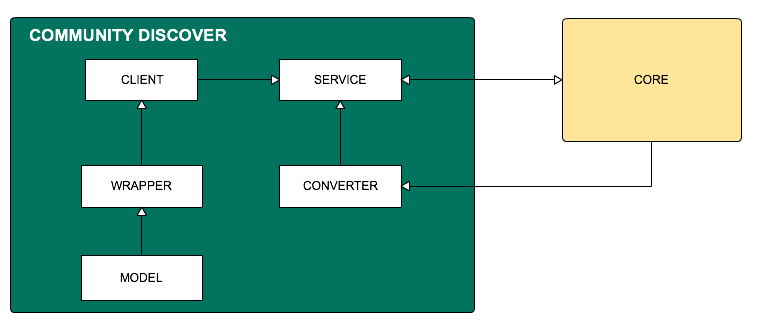
\includegraphics[scale=.6]{images/Figura4-2}
  \caption{\em Diagrama con la comunicación entre los componentes de \textit{Community Discover}}
  \label{fig:arq-im2}
\end{figure}

\section{Impacto en el modelo actual}

En esta sección se resumen los cambios que se han realizado en el Core de RBox para permitir el funcionamiento del ciclo de detección y persistencia de comunidades.

\subsection{\textit{Event}os}

Se han añadido dos tipos de eventos a RBox: \textit{mentioning} y \textit{replying}, como representación del modelo de interacciones que provee Twitter. No obstante, la implementación es genérica y son reutilizables en otra red social que utilice este tipo de eventos. Por ende, ambos son necesarios para contextualizar la herramienta a la red social que se analizará en el capítulo siguiente y poseen un valor de tipo String. Se han añadido versiones mutables e inmutables de ambos eventos.

\subsection{DAO}

Se han implementado la interfaz \textit{CommunityDAO} para el manejo de comunidades con esquemas relacionales a través de JDBC. Además, RBox no tenía implementado un mecanismo de persistencia en esquemas relacionales y solamente estaba enfocado en consumir información de este medio. Por lo tanto, para poder persistir las comunidades detectadas, ha sido necesario añadir esta funcionalidad y preparar \textit{statements} que faciliten el proceso de insertar comunidades y asociar usuarios a las comunidades a las que pertenecen. Se ha creado un DAO que facilite el acceso a los \textit{Item}s, ya que son parte fundamental de la generación de los \textit{\textit{Graph}Wrapper}.

\subsection{Extensions}

Se ha creado un nuevo módulo en RBox, que tiene que ver con el manejo de extensiones de funcionalidades. El funcionamiento está basado en transformaciones y encapsulamientos de datos, por lo que toda extensión, detección de comunidades incluída, debe definir sus propios servicios de transformación, que hereden de la interfaz Wrapper, desde y hacia 3-Ontology del esquema de datos en particular que cada extensión maneje (texto plano, xml, json, abstracto mediante objetos, entre otros).

En el caso particular de la extensión de detección de comunidades, se ha definido la interfaz \textit{CommunityExtension}, que utiliza, mediante \textit{Generics}, dos clases que heredan de la interfaz Wrapper para definir los servicios que esta extensión provee. En el segmento de código que muestra la Figura \ref{fig:arq-im3} está la definición de esta interfaz. En \textit{Community Discover}, la clase \textit{Community Discover}\textit{Client} es la que implementa esta interfaz, ya que es la que provee el servicio de detección y persistencia de comunidades.

\begin{figure}[H]
  \centering
  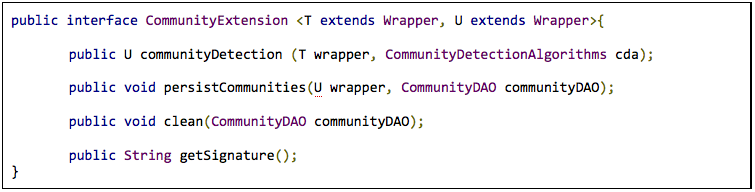
\includegraphics[scale=.6]{images/Figura4-3}
  \caption{\em Código que muestra la interfaz que debe implementar todo servicio de detección de comunidades.}
  \label{fig:arq-im3}
\end{figure}

Como se ha descrito, las modificaciones en el Core de RBox son menores y el mayor impacto y la lógica de los servicios y procesos reside en el componente \textit{Community Discover}. Luego, es hora de describir el proceso completo de comunicación entre los componentes mencionados en este capítulo.

\section{Comunicación entre componentes}

En esta sección se detalla el proceso de comunicación con todos los componentes ya descritos, a partir de un ejemplo de código que se muestra en la Figura \ref{fig:arq-im4}. En primer lugar, se obtiene una instancia de JDBCDAO y, con esta, se obtienen los eventos registrados en el medio persistente. Luego, se genera una instancia de GenericTrace utilizando como parámetro a los eventos obtenidos anteriormente. Posteriormente, se obtiene una lista de \textit{UserHistory}, agrupando los eventos para cada usuario.

\begin{figure}[H]
  \centering
  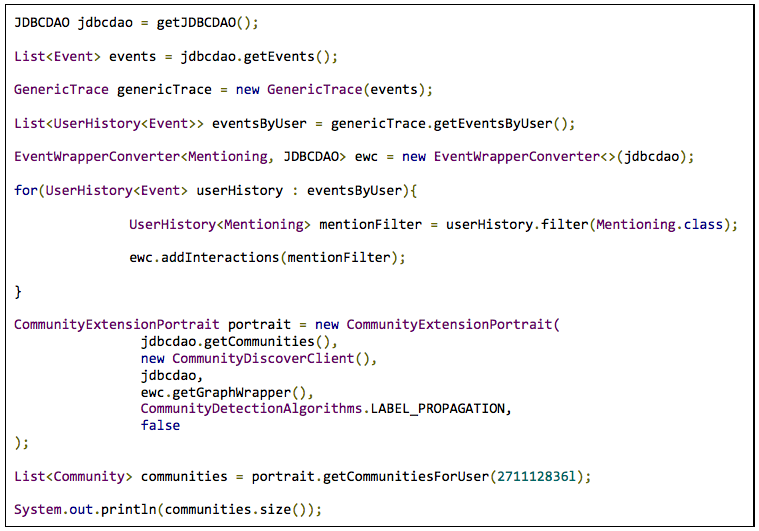
\includegraphics[scale=.6]{images/Figura4-4}
  \caption{\em Código que muestra la interacción entre los distintos componentes del servicio.}
  \label{fig:arq-im4}
\end{figure}


Una vez que se tiene el listado de \textit{User}History es necesario construir el encapsulador de eventos a un \textit{\textit{Graph}Wrapper}. Para esto se instancia un \textit{\textit{Event}WrapperConverter} utilizando como definición de Generics a la clase \textit{Mentioning}, y a JDBCDAO. Esto implica que los eventos que serán encapsulados son aquellos que sean de tipo \textit{Mentioning}.  Posteriormente, y para cada evento por usuario, se filtran los eventos para obtener sólo a aquellos que correspondan a \textit{Mentioning} y son esas interacciones las que se añaden al encapsulador. Cuando se tienen todos los eventos encapsulados, se crea el servicio \textit{Portrait} que provee \textit{Community Discover}. Para esto necesita:

\begin{enumerate}
  \item Todas las comunidades existentes en el sistema.
  \item Un cliente del servicio REST de detección de comunidades.
  \item Una instancia de JDBCDAO para permitir la persistencia de comunidades, según corresponda.
  \item Una instancia de \textit{\textit{Graph}Wrapper} que encapsule los eventos, que será enviado como \textit{request} al servicio de detección de comunidades.
  \item El algoritmo que se quiere que el servicio utilice al momento de detectar comunidades.
  \item Un valor booleano para determinar si se hace uso del primer nivel de \textit{community cache}. En otras palabras, si las comunidades se detectan siempre (\textit{true}) o solamente cuando no existan comunidades para un usuario (false).
\end{enumerate}

%TODO: CODIGO

Finalmente, se obtienen las comunidades para un usuario en particular. Si el usuario no tiene comunidades estas serán detectadas y se muestra la cantidad de comunidades a las que este usuario pertenece.

\section{Resumen}

En este capítulo se ha presentado el componente que se ha añadido a RBox para permitir la comunicación con el servicio de detección de comunidades presentado en el capítulo anterior. Además, se ha realizado una descripción componente a componente de cada uno de los submódulos de \textit{Community Discover}, el módulo REST que permite detectar comunidades en base a los eventos almacenados en lógica 3-Ontology. Luego, se ha analizado el impacto que la añadidura de este componente ha tenido sobre el \textit{core} de RBox ya desarrollado, identificando componentes restantes y añadiendo componentes nuevos para permitir el manejo de extensiones. Finalmente, se ha mostrado un ejemplo de integración de todos los componentes necesarios para realizar una detección de comunidades en base a un tipo de evento.

%--------Experimentación
%--------Daniel Ochoa John
%--------13/10/2014
\newcolumntype{L}[1]{>{\raggedright\let\newline\\\arraybackslash\hspace{0pt}}m{#1}}
\newcolumntype{C}[1]{>{\centering\let\newline\\\arraybackslash\hspace{0pt}}m{#1}}
\newcolumntype{R}[1]{>{\raggedleft\let\newline\\\arraybackslash\hspace{0pt}}m{#1}}

\chapter{Experimentación}
\label{cap:experimentacion}

En este capítulo se tratará el experimento realizado, ejecutado bajo todo el desarrollo tecnológico descrito en los Capítulos 3 y 4, que implica la manera de probar la hipótesis que este trabajo de tesis postula. En primer lugar, se describe el experimento realizado, considerando inputs, outputs y puntos de evaluación. Luego, se caracterizan los \textit{data\textit{set}} utilizados, describiendo su dominio y cuantificando su tamaño. Finalmente, se muestran los resultados obtenidos.

\section{Descripción del experimento}

En esta sección se describe el experimento que se ha realizado para cumplir con el objetivo general de este trabajo, que es probar que existe una mejora en la eficiencia de la recomendación al contar con un mecanismo de persistencia y reutilización de las comunidades detectadas al momento de recomendar contenido a los usuarios.

Para describir el experimento, es necesario mencionar que, en el flujo de datos propuesto por RBox, al momento de generar una recomendación es posible también obtener comunidades de usuarios con intereses similares (ver Figura \ref{fig:exp-im1}). El asunto tiene que ver con persistir la existencia de las comunidades y utilizarlas como un antecedente que haga más eficiente recomendaciones posteriores, por lo que el experimento buscará evaluar si persistir las comunidades detectadas en una primera recomendación acelera o no el proceso de recomendación en ejecuciones posteriores, sobre un sistema de recomendación generado con RBox.

\begin{figure}
  \centering
  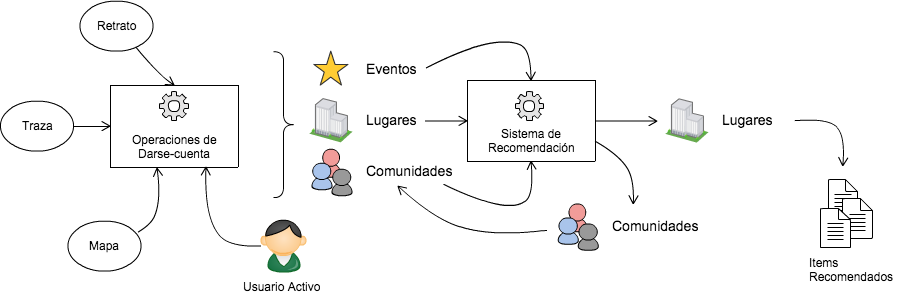
\includegraphics[scale=.5]{images/Figura5-1}
  \caption{\em Ciclo de recomendación en RBox.}
  \label{fig:exp-im1}
\end{figure}

Con este objetivo es que se ha generado un \textit{data\textit{set}} que será descrito en la sección siguiente. Sobre él se generará una recomendación de \textit{tags} considerando detección de comunidades, en tres escenarios que se detallarán más adelante. La detección de comunidades será llevada a cabo mediante los distintos algoritmos que provee el servicio, ya descrito en el Capítulo 4. Luego, se comparan los tiempos de ejecución considerando los escenarios de prueba.

\section{Caracterización de \textit{data\textit{set}}}

El \textit{data\textit{set}} que se ha utilizado para llevar a cabo el experimento ha sido obtenido a partir de la red social \textit{Twitter}. En concreto, se han generado un extractor de \textit{tweets} utilizando Ruby como lenguaje de programación. El extractor utiliza una gema llamada \textit{\textit{tweets}tream} para acceder a la Streaming API de \textit{Twitter}, permitiendo obtener el acceso a \textit{tweets} de índole público, en tiempo real. Cada uno de los \textit{tweets} es transformado a lógica 3-Ontology por el extractor y es persistido con la ayuda de un ORM\footnote{El mapeo objeto-relacional (en inglés \textit{Object Relational Mapping}, es una técnica que permite relacionar el diseño de clases de un diseño orientado a objetos, con un esquema de algún medio persistente.)} llamado Sequel\footnote{Fuentes y \textit{home} del proyecto en https://github.com/jeremyevans/sequel}.

El \textit{data\textit{set}} corresponde a una extracción dirigida de \textit{tweets}, orientado a la Copa Mundial de la Fifa Brasil 2014, para la que \textit{Twitter} ha promovido el uso de hash\textit{tags} particulares para cada país, como muestra la Tabla \ref{tab:exp-tab01}. Se ha hecho seguimiento a los comentarios que tengan que ver con los equipos sudamericanos que participan en la competición. La cuantificación de este \textit{data\textit{set}} se puede apreciar en la Tabla \ref{tab:exp-tab02}.  De cada uno de los \textit{tweets}, interesa saber de las siguientes interacciones:

\begin{enumerate}[I]
  \item \textbf{\textit{Mentioning}:} es el acto de referencia explícita, en un tweet, a un usuario. Denota un mensaje directo hacia otro usuario o una invitación a compartir una conversación respecto a un tema.
  \item \textbf{\textit{Tagging}:} es el acto de resaltar un concepto del mensaje utilizando un \textit{hashtag}. Generalmente, marca un tópico relevante que conlleva un interés particular del usuario, que motiva y fundamenta el contenido que ha compartido en la red social.
  \item \textbf{\textit{Replying}:} es el acto de replicar con un tweet la aseveración, comentario o mención de otro usuario.
\end{enumerate}

\begin{table}[H]
  \begin{center}
    \caption{Hash\textit{tags} particulares de cada país durante la copa mundial de la FIFA en \textit{Twitter}.}
    \label{tab:exp-tab01}
      \begin{tabular}{|L{4cm}|L{4cm}|}
        \hline
        \textbf{\textit{Hashtag}} & \textbf{País}\\ \hline
         \#CHI & Chile.\\ \hline
         \#BRA & Brasil.\\ \hline
         \#ARG & Argentina.\\ \hline
         \#COL & Colombia. \\ \hline
         \#ECU & Ecuador. \\ \hline
      \end{tabular}
  \end{center}
\end{table}

\begin{table}[H]
  \begin{center}
    \caption{Cuantificación del \textit{data\textit{set}} de la copa mundial de la FIFA.}
    \label{tab:exp-tab02}
      \begin{tabular}{|L{4cm}|L{4cm}|}
        \hline
        \textbf{Medida} & \textbf{Valor}\\ \hline
         \textit{Event} & 445.342\\ \hline
         \textit{Item} & 23.739\\ \hline
         \textit{User} & 91489\\ \hline
         \textit{Tweets} & 64.120\\ \hline
         \textit{Mentioning} & 92.519\\ \hline
         \textit{Tagging} & 349.577\\ \hline
         \textit{Replying} & 3.246\\ \hline
      \end{tabular}
  \end{center}
\end{table}

Como primer análisis, se considera el top 3 de usuarios que han compartido más \textit{tweets}, que incluyen menciones a otros usuarios (ver Tabla \ref{tab:exp-tab02}). Si se considera a estos usuarios, como activos, el grafo que representa sus interacciones se puede apreciar en las Figuras \ref{fig:exp-im2}, \ref{fig:exp-im3} y \ref{fig:exp-im4}, respectivamente. Si se realiza una detección de comunidades sobre el grafo de interacciones para estos usuarios, mediante, por ejemplo, del método \textit{Multilevel} (ver Capítulo 3), las comunidades detectadas pueden apreciarse en las Figuras \ref{fig:exp-im5}, \ref{fig:exp-im6} y \ref{fig:exp-im7}, respectivamente.

\begin{table}[H]
  \begin{center}
    \caption{Top 3 de usuarios con mas \textit{tweets} que consideran menciones a otros usuarios.}
    \label{tab:exp-tab02}
      \begin{tabular}{|L{4cm}|L{4cm}|}
        \hline
        \textbf{\textit{User} (Alias)} & \textbf{Nº de Menciones}\\ \hline
         539210296 (1) & 95\\ \hline
         2320149583 (2) & 85\\ \hline
         2463599637 (3)& 69\\ \hline
      \end{tabular}
  \end{center}
\end{table}

\begin{figure}
  \centering
  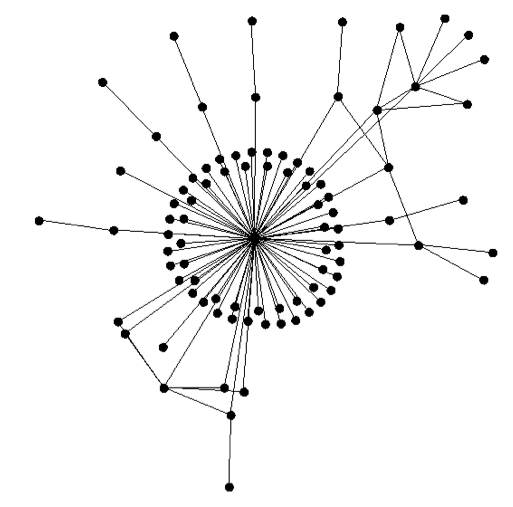
\includegraphics[scale=.7]{images/Figura5-2}
  \caption{\em Grafo de interacciones generado por el usuario 1.}
  \label{fig:exp-im2}
\end{figure}

\begin{figure}
  \centering
  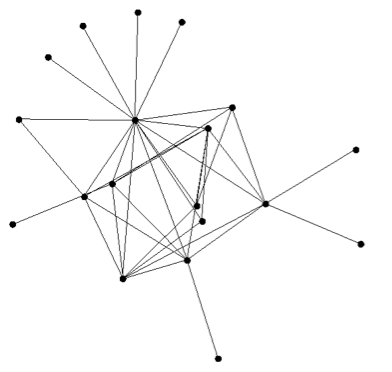
\includegraphics[scale=.7]{images/Figura5-3}
  \caption{\em Grafo de interacciones generado por el usuario 2.}
  \label{fig:exp-im3}
\end{figure}

\begin{figure}
  \centering
  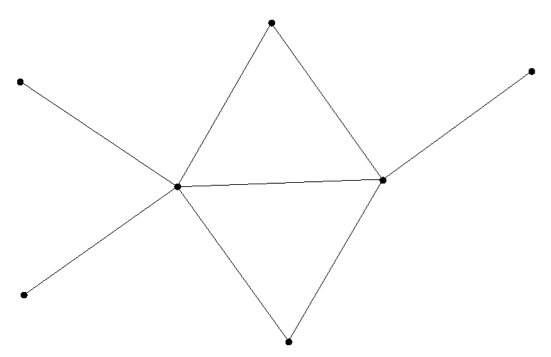
\includegraphics[scale=.7]{images/Figura5-4}
  \caption{\em Grafo de interacciones generado por el usuario 3.}
  \label{fig:exp-im4}
\end{figure}

\begin{figure}
  \centering
  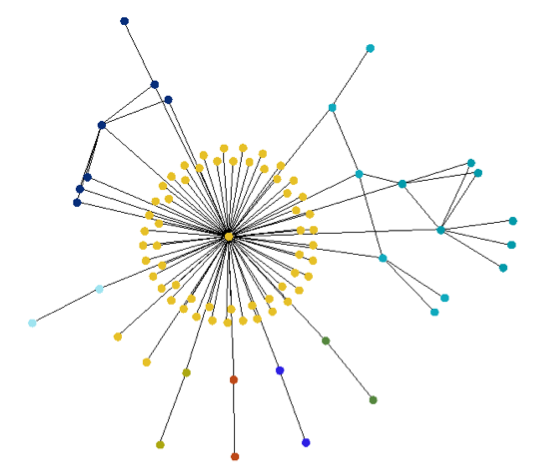
\includegraphics[scale=.7]{images/Figura5-5}
  \caption{\em Comunidades detectadas en base al grafo de interacciones generado por el usuario 1.}
  \label{fig:exp-im5}
\end{figure}

\begin{figure}
  \centering
  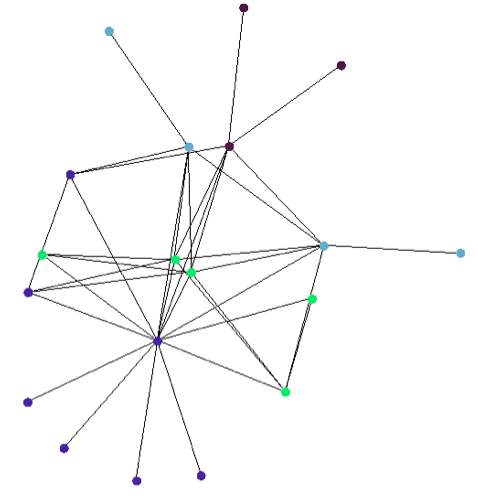
\includegraphics[scale=.7]{images/Figura5-6}
  \caption{\em Comunidades detectadas en base al grafo de interacciones generado por el usuario 2.}
  \label{fig:exp-im6}
\end{figure}

\begin{figure}
  \centering
  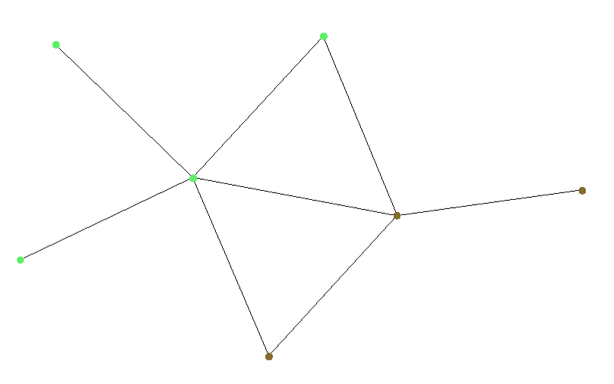
\includegraphics[scale=.7]{images/Figura5-7}
  \caption{\em Comunidades detectadas en base al grafo de interacciones generado por el usuario 3.}
  \label{fig:exp-im7}
\end{figure}

\section{Resultados}

Para experimentar con un proceso de recomendación utilizando comunidades, se ha implementado un algoritmo de recomendación de tags, cuyo objetivo es retornar los top N \textit{tags} con mayor ocurrencia en una comunidad. Para generar las comunidades, se considera el evento \textit{Mentioning}, se han omitido los registros que consideran a menos de diez menciones hacia otros usuarios para eliminar la generación de comunidades pequeñas. La distribución de \textit{mentions} del \textit{dataset}, por rango, se puede apreciar en la Tabla \ref{tab:exp-tab03}.

De cada uno de los rangos se han seleccionado aleatoriamente dos usuarios, con el objetivo de analizar los tiempos requeridos para obtener una recomendación, considerando el mecanismo de \textit{community cache} como eje al momento de persistir las comunidades que ellos generan mediante sus interacciones en la red social. 

Los escenarios de prueba son diseñados para simular el comportamiento de la \textit{community cache} y todos tienen en consideración diez iteraciones, utilizando tres métodos de detección de comunidades, \textit{Multilevel}, \textit{LeadingEigenvector} e \textit{Infomap}. Las consideraciones particulares de los escenarios tienen relación con el estado inicial del medio persistente, la estrategia de caché y el estado final del medio persistente, estos son:

\begin{enumerate}
	\item \textbf{Escenario 1 (E1)}: Considera un medio persistente inicial sin comunidades, la estrategia de persistencia es mediante el primer nivel de \textit{community cache} y al final de cada ciclo de iteraciones, el medio persistente es reiniciado.
	\item \textbf{Escenario 2 (E2)}: Considera un medio persistente inicial sin comunidades, la estrategia de persistencia es mediante el segundo nivel de \textit{community cache} y al final de cada ciclo de iteraciones, el medio persistente es reiniciado.
	\item \textbf{Escenario 3 (E3)}: Considera un medio persistente inicial sin comunidades, la estrategia de persistencia es mediante el segundo nivel de \textit{community cache} y al final de cada ciclo de iteraciones se conserva el medio persistente.
\end{enumerate}

El experimento considera la ejecución de cada uno de los escenarios, para todos los usuarios, detectando comunidades mediante los tres métodos. La referencia de los usuarios seleccionados y sus interacciones mediante mentions se puede apreciar en la Tabla \ref{tab:exp-tab04}, se les ha asignado un alias que permitirá identificarlos de manera abreviada en los análisis venideros.

\begin{table}[H]
  \begin{center}
    \caption{Distribución de eventos \textit{mention} en el \textit{dataset}.}
    \label{tab:exp-tab03}
      \begin{tabular}{|L{4cm}|L{4cm}|}
        \hline
        \textbf{Rango} & \textbf{Menciones}\\ \hline
         [10 - 25) & 520\\ \hline
         [25 - 50) & 34\\ \hline
         [50 - 75) & 5\\ \hline
         [75 - 100) & 2\\ \hline
      \end{tabular}
  \end{center}
\end{table}

\begin{table}[H]
  \begin{center}
    \caption{Usuarios seleccionados, número de menciones y alias para experimento.}
    \label{tab:exp-tab04}
      \begin{tabular}{|L{4cm}|L{4cm}|L{4cm}|}
        \hline
        \textbf{Usuario} & \textbf{Menciones} & \textbf{Alias} \\ \hline
         1360359360 & 12 & U1\\ \hline
         577741173 & 24 & U2\\ \hline
         2544108592 & 49 & U3\\ \hline
         301461393 & 27 & U4\\ \hline
         2463599637 & 69 & U5\\ \hline
         525904011 & 54 & U6\\ \hline
         539210296 & 95 & U7\\ \hline
         2320149583 & 85 & U8\\ \hline
      \end{tabular}
  \end{center}
\end{table}

La Figura \ref{fig:exp-im8} muestra el comportamiento de los tiempos requeridos para realizar una recomendación al usuario Ui, en adelante Tr, en E1. Se puede apreciar que Tr experimenta un descenso progresivo a través de las iteraciones y en la iteración final Tr siempre es menor que en la primera iteración. Esto es ocasionado por la condición de inicialización del medio persistente, como no hay comunidades para el usuario activo, el tiempo es utilizado en detectar, persistir y relacionar comunidades. Como está activado el primer nivel de cache, no es necesario detectar comunidades en iteraciones posteriores, por lo que el tiempo de estabilización, entre la segunda iteración y la novena, es principalmente utilizado por el sistema de recomendación propiamente tal, y por la validación de caché.

\begin{figure}[H]
  \centering
  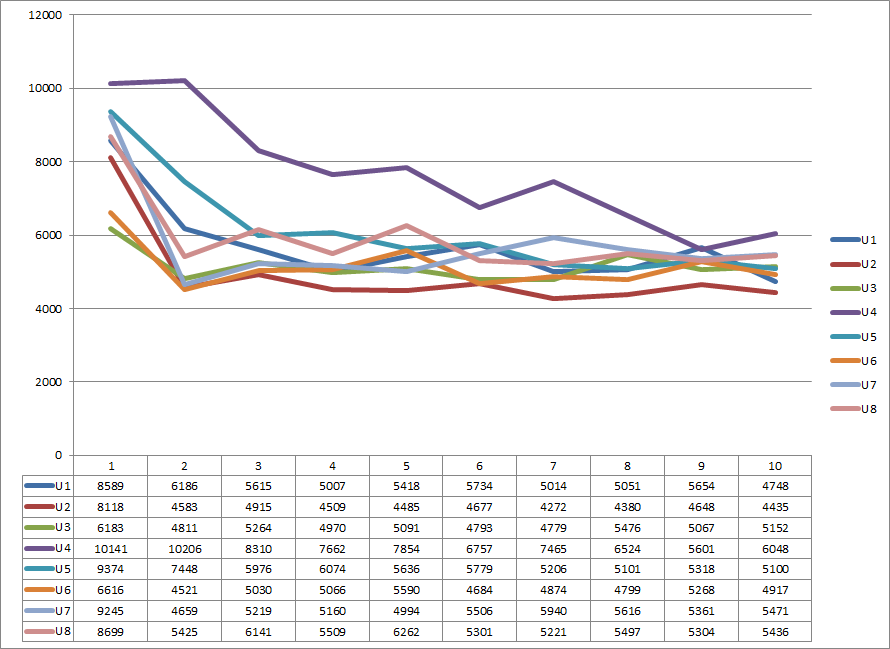
\includegraphics[scale=.7]{images/Figura5-8}
  \caption{\em Tiempos promedio (ms) requeridos para realizar una recomendación a Ui en E1.}
  \label{fig:exp-im8}
\end{figure}

La Figura \ref{fig:exp-im9} muestra el comportamiento de Tr en E2. Se puede apreciar que el descenso de Tr es muy marcado entre la primera y la segunda iteración. La estabilización de Tr parece ocurrir antes, debido a que el segundo nivel de cache controla las operaciones de persistencia innecesarias. Existen anomalías en la curva de U1 entre las iteraciones 7 y 9 debido a una sobrecarga no controlada de procesamiento mientras estaba ejecutándose la detección de comunidades por el método multilevel. Se refleja en la curva debido a la utilización de promedios para agrupar los tiempos de ejecución de los tres métodos. No obstante, la Figura \ref{fig:exp-im10} muestra el gráfico específico para U1, donde se puede apreciar explícitamente el peak de Multilevel entre las mencionadas iteraciones.

\begin{figure}[H]
  \centering
  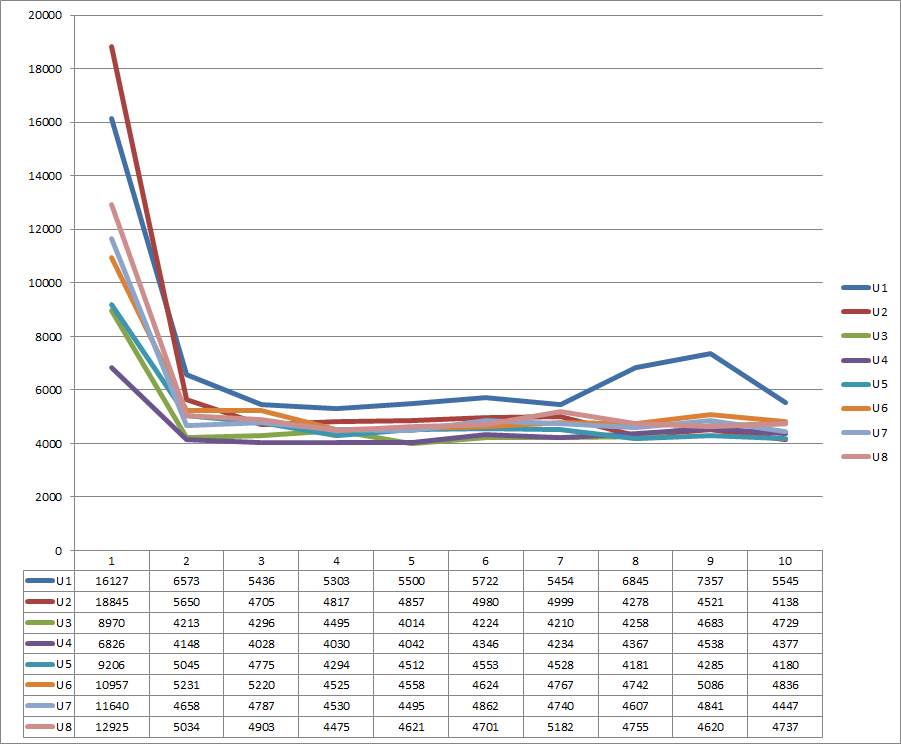
\includegraphics[scale=.7]{images/Figura5-9}
  \caption{\em Tiempos promedio (ms) requeridos para realizar una recomendación a Ui en E2.}
  \label{fig:exp-im9}
\end{figure}

\begin{figure}[H]
  \centering
  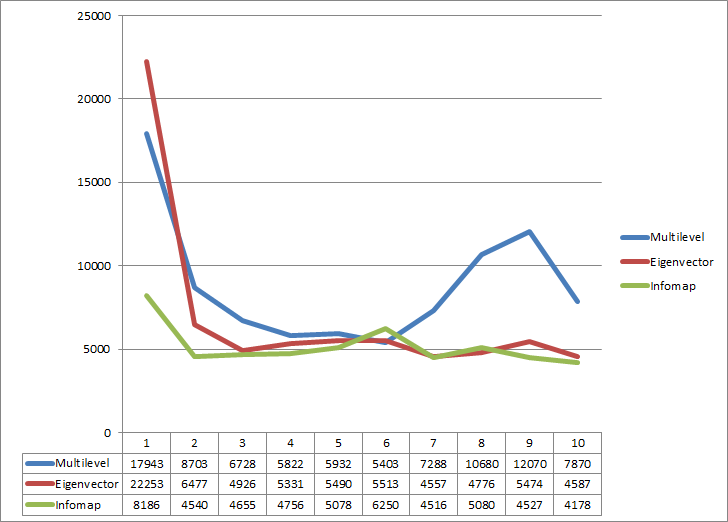
\includegraphics[scale=.7]{images/Figura5-10}
  \caption{\em Tr (ms) para U1 en E2.}
  \label{fig:exp-im10}
\end{figure}

La Figura \ref{fig:exp-im11} muestra el comportamiento de Tr en E3. La principal diferencia radica en la pequeña variación en los tiempos entre una iteración y otra. Como es la tónica, se aprecia un descenso en Tr a partir de la segunda iteración. La variación de los tiempos tiene que ver con que, como una de las condiciones de E3 es no limpiar el medio persistente al fin de cada secuencia de iteraciones, el sistema de cache tiene comunidades donde comparar y evaluar si corresponde su persistencia.

\begin{figure}[H]
  \centering
  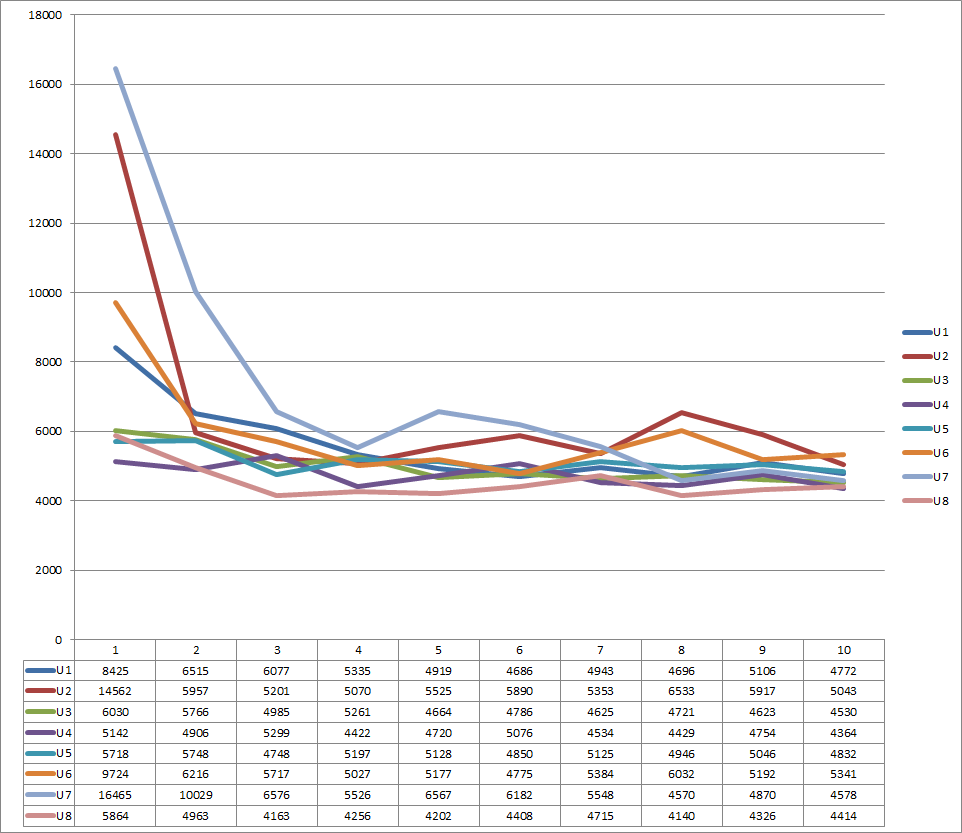
\includegraphics[scale=.7]{images/Figura5-11}
  \caption{\em Tiempos promedio (ms) requeridos para realizar una recomendación a Ui en E3.}
  \label{fig:exp-im11}
\end{figure}

La Figuras \ref{fig:exp-im12}, \ref{fig:exp-im13} y \ref{fig:exp-im14} muestran la diferencia que existe, para cada uno de los usuarios seleccionados, en Tr en tres casos: en la primera iteración (T0) , en la última (T10) y la línea del promedio (AVG), para todos los escenarios, respectivamente. Se puede apreciar que, para todos los usuarios y en todos los escenarios, siempre la primera iteración toma más Tr que la última, y más aún, que el promedio de iteraciones es menos costoso que la primera iteración. 

\begin{figure}[H]
  \centering
  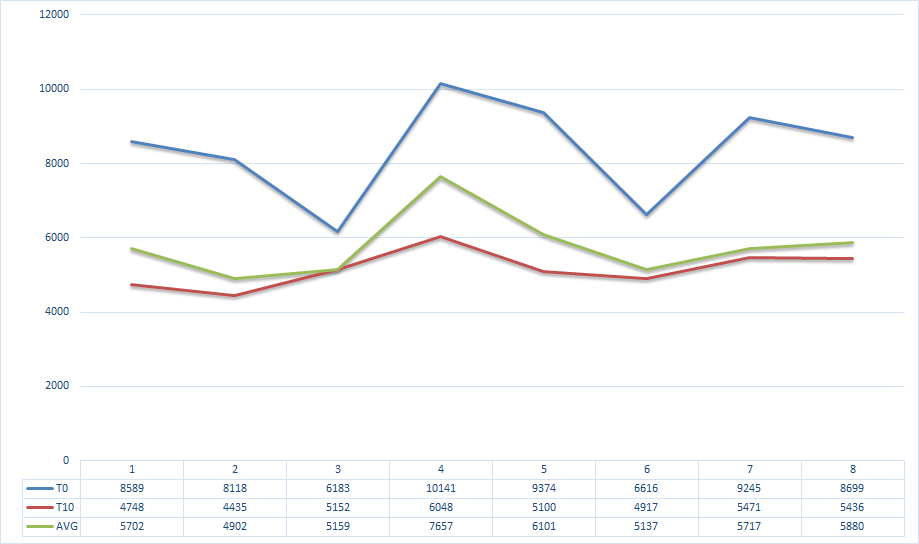
\includegraphics[scale=.7]{images/Figura5-12}
  \caption{\em Tr (ms) para T0, T10 y AVG en E1.}
  \label{fig:exp-im12}
\end{figure}

\begin{figure}[H]
  \centering
  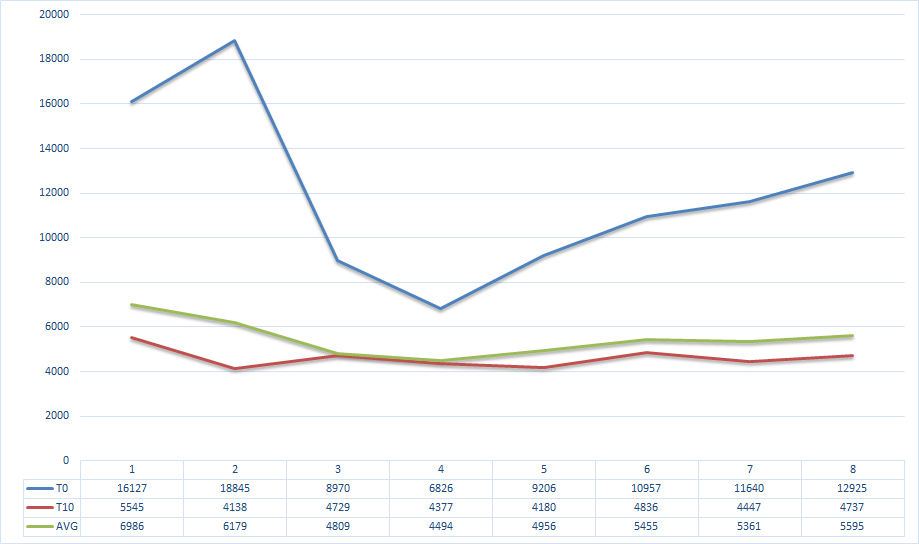
\includegraphics[scale=.7]{images/Figura5-13}
  \caption{\em Tr (ms) para T0, T10 y AVG en E2.}
  \label{fig:exp-im13}
\end{figure}

\begin{figure}[H]
  \centering
  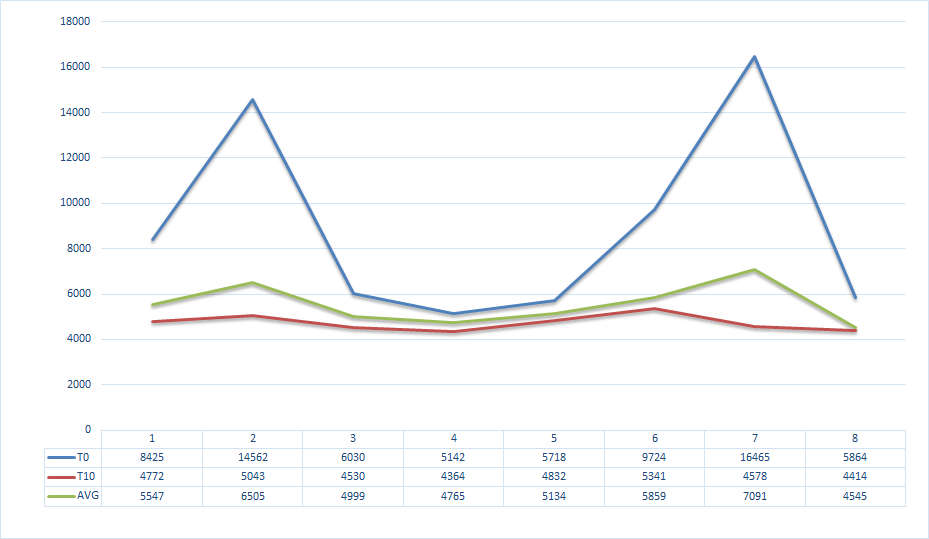
\includegraphics[scale=.7]{images/Figura5-14}
  \caption{\em Tr (ms) para T0, T10 y AVG en E3.}
  \label{fig:exp-im14}
\end{figure}

La Tabla \ref{tab:exp-tab05} muestra el análisis de varianza de factor simple (ANOVA) para Tr en E1 y E2, considerando T0 y T10 para todos los usuarios. E3 se ha dejado fuera de este análisis ya que cada iteración no es completamente independiente de otra. Se puede apreciar que F es mayor que F crit en los ambos casos, por lo que la reducción de tiempo es significativa y no dependiente de condiciones azarosas.

\begin{table}[H]
  \begin{center}
    \caption{Análisis de varianza de factor simple.}
    \label{tab:exp-tab05}
      \begin{tabular}{|L{1cm}|L{4cm}|L{4cm}|L{4cm}|}
        \hline
        \textbf{E} & \textbf{F} & \textbf{P} & \textbf{F crit} \\ \hline
         1 & 39,15251 & 2,1E-05 & 4,60011\\ \hline
         2 & 26,95112 & 0,000137 & 4,60011\\ \hline
      \end{tabular}
  \end{center}
\end{table}



\section{Resumen}

En este capítulo se ha descrito y presentado los resultados del experimento aplicado con el propósito de conseguir el objetivo general planteado en este trabajo de Tesis. En primer lugar, se ha descrito detalladamente el experimento realizado, con sus componentes y distintos escenarios. Luego, se ha caracterizado el \textit{data\textit{set}} utilizado para realizar las pruebas, describiendo el mecanismo de extracción, construcción, persistencia y cuantificación del tamaño de información contenida. Posteriormente, se han mostrado ejemplos de detección de comunidades utilizando el \textit{data\textit{set}} descrito. Finalmente, se han expuesto los resultados de la experimentación, logrando reducir el tiempo requerido para realizar una recomendación, mediante el uso del \textit{framework} y componentes descritos en los Capítulos 3 y 4.

%--------Conclusiones
%--------Daniel Ochoa John
%--------20/07/2014
\newcolumntype{L}[1]{>{\raggedright\let\newline\\\arraybackslash\hspace{0pt}}m{#1}}
\newcolumntype{C}[1]{>{\centering\let\newline\\\arraybackslash\hspace{0pt}}m{#1}}
\newcolumntype{R}[1]{>{\raggedleft\let\newline\\\arraybackslash\hspace{0pt}}m{#1}}

\chapter{Conclusiones}
\label{cap:conclusiones}

En este capítulo, se expone respecto a las conclusiones obtenidas del trabajo de tesis desarrollado. En primer lugar, se describe y evidencia el cumplimiento de los objetivos específicos. Luego, se explicitan los aportes realizados tanto al área de los SR, como al área de detección de comunidades. Posteriormente, se presentan aquellas aristas de investigación futuras, nacidas en base al trabajo aquí expuesto. Para terminar, se enuncian reflexiones finales en relación al presente trabajo de tesis.

\section{Respecto a los objetivos específicos}

Con respecto a los objetivos específicos definidos para el trabajo de tesis:

\begin{enumerate}
  \item Seleccionar técnicas y/o algoritmos que permitan la detección de comunidades. \newline

  Se evaluaron distintas alternativas de implementación de algoritmos para la detección de comunidades, en el Capítulo 3, en la sección 3.6 se definen aquellos algoritmos que permiten la detección de comunidades (Blondel, Guillaume, Lambiotte, & Lefebvre, 2008; Raghavan, Albert, & Kumara, 2007; Newman, 2006; Rosvall & Bergstrom, 2008; Traag & Bruggeman, 2009).\newline

  Estos algoritmos han sido implementados desde una librería llamada python-igraph. Esta librería ha sido construída en base a un kernel en C, y cuenta con abstracciones hacia ruby, R y python. Precisamente es esta última abstracción la que se utiliza para desarrollar un servicio de tipo REST, al que RBox se conecta, permitiendo la detección de comunidades. Uno de los algoritmos es de tipo no determinista al aplicar un método de Label Propagation, el cual fue incorporado al servicio solamente para disponibilizar todos aquellos algoritmos que igraph provee y no fue utilizado para las posteriores pruebas del sistema. \newline

  \item Definir la arquitectura del servicio que se añadirá a RBox, junto con un proceso de encapsulamiento de los datos del \textit{framework} para estandarizar el consumo del servicio. \newline

  En el Capítulo 3, se describe la arquitectura del servicio que se ha construido para detectar comunidades, que es diagramada en la Figura \ref{fig:serv-im1} muestra el diagrama de la arquitectura definida. El servicio está compuesto de distintas piezas de \textit{software} que permiten recibir, interpretar, calcular y transformar la información desde un formato orientado a vértices y nodos hacia una comunidad. \newline

  Su añadidura a RBox se define en el Capítulo 4, donde se describe una pieza que permite comunicarse con servicios de tipo REST.  En particular, en la sección 4.4 se describe el mecanismo que permite manejar la respuesta del servicio REST hacia una representación de comunidad definida en la 3-Ontology. Este mecanismo (ver Figura \ref{fig:arq-im2}) comprende una comunicación desde una pieza de encapsulamiento de las interacciones almacenadas en el modelo de la 3-Ontology (Wrapper) hasta el consumo  del servicio y reconversión de las comunidades detectadas hacia el esquema. \newline

  Por otra parte, el proceso de encapsulamiento de la información hacia el servicio, forma parte de la pieza Wrapper de \textit{Community Discover}. Esta pieza permite transformar desde el esquema de la 3-Ontology hacia un esquema de grafos con el objetivo de enviarlo como parámetro al momento de consumir el servicio. \newline

  \item Implementar y añadir a RBox un servicio que detecte y persista las comunidades, \textit{community cache}, a partir de los datos encapsulados. \newline

  En el Capítulo 4, se describe una implementación de \textit{Portrait} que considera la detección y persistencia de las comunidades encapsuladas a través del servicio de detección de comunidades. Esta pieza forma parte de \textit{Community Discover} y ha sido añadida como una extensión del Core de RBox. En la Figura \ref{fig:arq-im1} se muestra el diseño de la arquitectura en la que este servicio está inserto. \newline

  El servicio posee un mecanismo llamado \textit{community cache}, que consta de dos niveles. En un primer nivel, determina si la detección y persistencia se realiza únicamente cuando el usuario activo no tiene comunidades asociadas. En el segundo nivel, tiene un mecanismo de control respecto a la persistencia, por cuanto se toma en cuenta el hecho de que la comunidad ya forma parte del modelo de la 3-Ontology, considerando el conjunto de usuarios que la forman. \newline

  El servicio toma como antecedentes a todas las comunidades existentes en el sistema, el cliente del servicio REST de detección de comunidades, una instancia del DAO de RBox para permitir la persistencia de comunidades, una instancia de \textit{\textit{Graph}Wrapper} que encapsule los eventos, que será enviado como \textit{request} al servicio de detección de comunidades, el algoritmo que se utilizará para detectar comunidades, un valor booleano para determinar si se hace uso del primer nivel de \textit{community cache}. \newline

  \item Implementar un algoritmo de recomendación utilizando la información de las comunidades como antecedente. \newline

  En el Capítulo 5 se muestran distintos ejercicios de recomendación basados en las comunidades de un usuario activo, considerando un algoritmo de recomendación de los top N \textit{tags} más utilizados en una comunidad. Los que se busca es medir la performance de la generación de recomendación considerando el tiempo necesario para realizar las operaciones de encapsulación, consumo, transformación y persistencia para detectar comunidades, evaluando si el mecanismo de community-cache existente es realmente una medida de reducción del tiempo necesario para recomendar detectando comunidades a un usuario activo, considerando aquellas comunidades detectadas como una retroalimentación a recomendaciones posteriores. \newline

  \item Analizar tiempos de respuesta obtenidos al monento de generar recomendaciones, con la finalidad de confirmar o descartar la hipótesis planteada. \newline

  En la Sección 5.3 se exponen conclusiones respecto a los resultados obtenidos de la experimentación. Se marcan las diferencias entre la partida “en frío” de una recomendación y la detección de comunidades cuando esta se fuerza para cada recomendación. Los ejercicios han sido realizados considerando tres estrategias distintas de detección de comunidades, diez iteraciones de recomendación y tres escenarios. \newline

  Estos escenarios son: primero, detectando y persistiendo comunidades solamente cuando el usuario no tenga comunidades asociadas; segundo y tercero, detectando y persistiendo comunidades siempre, para cada iteración. Con la salvedad de que el tanto el primer como el segundo escenario consideran a un medio persistente vacío entre la ejecución de distintas estrategias. \newline

  Los resultados del primer caso de pruebas muestran que en la primera iteración el tiempo que se requiere para obtener la recomendación siempre es mayor que en las iteraciones posteriores. Los resultados del segundo caso de pruebas muestran el funcionamiento de la \textit{community cache}, ya que el \textit{framework} no persiste aquellas que ya existen, eliminando duplicidad. Finalmente, en el tercer caso de pruebas el tiempo necesario para otorgar la primera recomendación se ha reducido, en general, ya que existen comunidades que ya han sido detectadas en iteraciones precedentes. \newline

  \item Publicar los resultados en una revista de la especialidad. \newline

  Están en desarrollo dos publicaciones en revistas de la especialidad. Una relacionada con el aporte científico de la mejora en eficiencia de los SR usando el mapping de la 3-Ontology el concepto de \textit{community cache}. La segunda publicación estará basada en la arquitectura que permite construir el \textit{framework} que retroalimenta el esquema de la 3-Ontology con las comunidades detectadas, reduciendo así el tiempo requerido para volver a realizar la misma recomendación. \newline

\end{enumerate}

\section{Aportes del trabajo}

En primer lugar, este trabajo provee un \textit{framework} de detección de comunidades en base a una arquitectura unificada de componentes. Esto facilita la posibilidad de incorporar nuevos métodos de detección de comunidades al servicio presentado, o bien, desarrollar encapsuladores para otro servicio o API que provea prestaciones similares. Se desprende también de lo recién mencionado que, con la incorporación de un API para implementar clientes de tipo REST, se incorpora a RBox la posibilidad de consumir servicios de distinta índole, como análisis de sentimientos, geolocalización o \textit{named entity recognition}. Además, y como la arquitectura orientada a servicios desarrollada en este trabajo es extensible, se pueden incorporar elementos y algoritmos de análisis de redes sociales para el uso y disposición de los sistemas de recomendación que sean implementados en RBox.

En segundo lugar, se ha incorporado a RBox un mecanismo de recomendación basado en comunidades que se retroalimenta de las recomendaciones hechas en el pasado como una cache. Esto permite mejoras tanto en los tiempos necesarios para recomendar contenido a los usuarios, desde la perspectiva de las comunidades a las que pertenecen, como en el control de duplicidad de comunidades que puedan existir, ya que no se persistirá dos veces una misma comunidad.

En tercer lugar, el \textit{framework} que permite transformar las interacciones sociales en grafos de interacciones es un modelo flexible, que permite construir comunidades desde distintos puntos de vista y considerando diferentes interacciones existentes en un dominio en particular. En el caso de este trabajo de tesis, las comunidades fueron construidas a partir de las interacciones ocasionadas por las menciones de los usuarios en \textit{Twitter}. No obstante, nada impide construir comunidades distintas considerando otras interacciones, como \textit{replying}, \textit{following} y \textit{retweeting}.

\section{Trabajos futuros}

En este trabajo se propone e implementa una arquitectura que permite retroalimentar las comunidades en un esquema 3-Ontology a partir de recomendaciones basadas en un usuario activo.  No obstante, simplemente se comienza la exploración de la dimensión de la comunidad y tras esto se vislumbran los siguientes trabajos futuros:

\begin{itemize}
  \item Incorporar un servicio, plugin o extensión que permita realizar un análisis de redes sociales, orientadas a la dimensión de la comunidad. Permitiendo enriquecer la recomendación en base a la confianza y popularidad de los usuarios que componen las comunidades.
  \item Explorar la dimensión de los lugares, mediante la incorporación de un servicio, plugin o extensión que explicite los tipos de información espacial utilizados en los sistemas de recomendación.
  \item Definir una extensión de la arquitectura que permita obtener granularidad y detalle en los datos de las comunidades. Como por ejemplo obtener, en tiempo real desde la fuente de información (sea API, \textit{crawling}, \textit{scrapping}, entre otras), mayor cantidad de datos en relación a un usuario en particular. Esto completaría aún más la construcción dinámica de comunidades en base a las distintas interacciones o tipos de eventos.
  \item Construir un \textit{dashboard} o herramienta exploratoria que facilite la navegación por los contenedores de sentido de la 3-Ontology, permitiendo a analistas de \textit{social media} y personas interesadas, la toma de decisiones en base al comportamiento e interacciones presentes en el conjunto de datos.
  \item Construir, a partir de RBox, observatorios de ciertas fracciones de la Web, permitiendo la definición dinámica de extractores de información a un esquema 3-Ontology. Esto permitiría alimentar a RBox con datos de distintas fuentes en base al interés que la entidad que provee recomendaciones defina.
\end{itemize}

\section{Reflexiones Finales}

Este trabajo de tesis pone fin a dos años de esfuerzo y dedicación que han supuesto un crecimiento sustancial en mi calidad como profesional y como investigador. Las asignaturas del programa de Magíster en Ingeniería Informática de la Universidad son un buen complemento a la formación inicial obtenida en pregrado. Personalmente, en el año 2011, me titulé de Ingeniero de Ejecución en Computación e Informática y, debido al trabajo y la dedicación puesta en la carrera, fui beneficiado por una media beca de arancel para ingresar al programa de Magíster. Esto ha sido un desafío no menor, ya que típicamente el programa está diseñado para que sea completado por ingenieros civiles (con los dos años extra de formación que implica ese plan de estudios). Sin embargo, la motivación principal ha sido sentar un precedente y demostrar a todos los estamentos (sobre todo a mis colegas de carrera) que las capacidades son transversales a la carrera que uno estudie y la motivación que se requiere para completar un programa de postgrado viene principalmente por las aspiraciones del estudiante, a pesar de que muchas veces el trabajo no es buen amigo del estudio y las empresas no están plenamente conscientes de los beneficios que trae para ellos el contar con un estudiante de postgrado en su equipo de ingenieros. En ese sentido, el desafío que hay que asumir ahora es el de abrir camino a las generaciones que vienen con el hecho de intentar cambiar la tendencia nacional, demostrando pragmáticamente que el rendimiento y el conocimiento de un profesional con postgrado es aporte más que relevante tanto para la línea de innovación de las empresas, como para la línea de negocios.

El programa de postgrado, en términos profesionales, ha sido un aporte significativo. A pesar de que muchas veces sus contenidos no están actualizados en base a las actuales tendencias de la profesión, si me ha instado a no dejar de estudiar y estar a la vanguardia en un mundo tremendamente competitivo, en el que las tecnologías, patrones, arquitecturas y tendencias no viven más de dos años. Se destaca, sin lugar a dudas, el conocimiento adquirido al trabajar a la par de compañeros y profesores talentosos, en especial con aquellos que pertenecen al grupo FONDEF, que lidera el Dr. Edmundo Leiva y en el cual participé. La necesidad de entregar, en este trabajo, una solución tecnológica cuya calidad estuviera a la altura de los distintos componentes incorporados ya al proyecto, ha sido otra manera de impulsar el aprendizaje, la lectura y mejorar progresivamente mis habilidades en diseño y desarrollo de soluciones tecnológicas que están inmersas en un contexto de uso constante y no quedan guardadas en la estantería.

El haber trabajado en una tesis enfocada a \textit{social media} ha supuesto la continuación de una inquietud que nace en el desarrollo de mi memoria de pregrado y que sentí inconclusa. Me ha permitido investigar, analizar y conocer distintos aspectos de un tema que hoy mueve y tendencia fuertemente el uso de Internet como plataforma fundamental para la masificación de contenidos y las relaciones sociales mediada por tecnología. Esta tendencia está manteniéndose en el tiempo y alcanzando distintas aristas, desde meramente compartir información, hasta proveer, con ayuda de la nube, distintos servicios de análisis de tópicos y comunidades enfocadas al \textit{business intelligence} y el cultivo de la inteligencia colectiva. En mi opinión, lo colectivo y lo comunitario son los negocios del mañana y el aplicar los conocimientos involucrados en esta tesis puede contribuir, aunque sea en parte, a esta tendencia.


% ----------------------------------------------------------
% ----------- TERCERA PARTE --------------------------------
% \backmatter %Elimina la numeración
% ### Bibliografía de este documento ###
\nocite{*}
\bibliographystyle{apa-good}
\bibliography{TesisMagister}

% ----------------------------------------------------------
% ----------- CUARTA PARTE ---------------------------------
\appendix
\addappheadtotoc %agregar Apéndice al índice
\noappendicestocpagenum %quitar número de páginas a los apéndices
% ### ANEXOS ###
%--------Anexo 1
%--------Daniel Ochoa John
%--------13/10/2014

\chapter{Glosario}

\begin{itemize}
	\item \textbf{Colaborativo}: Proceso de interacción humana donde las personas realizan continuamente una dualidad de funciones entre cliente y realizador, para realizar un trabajo colectivo. El trabajo colaborativo puede ser explícito o implícito como ocurre en la Web 2.0.
	\item \textbf{Comunidad}: Conjunto de indivíduos que poseen intereses similares y que interactúan entre sí con mayor frecuencia que con otras comunidades.
	\item \textbf{Detección de comunidades}: Conjunto de técnicas que permiten explicitar las agrupaciones entre indivíduos basándose en el conjunto de interacciones llevadas a cabo por los integrantes de un contexto social. Es considerada parte de la teoría de grafos y muchas de sus aplicaciones en la social media tienen que ver con el \textit{clustering} y catalogación de grupos de interés.
	\item \textbf{Endpoint}: En el mundo de los servicios Web, un endpoint es la dirección absoluta en la que un servicio está disponible. Esta dirección debe ser conocida por el cliente del servicio y no necesariamente deben pertenecer al mismo sistema computacional. En el diseño de servicios moderno, la nomenclatura para los endpoints está regida por REST.
	\item \textbf{Filtrado basado en contenido}: Proporciona recomendaciones mediante la comparación de las preferencias de un usuario en el pasado, recomendando aquellos ítems que son similares.
	\item \textbf{Filtrado colaborativo}: Proporciona recomendaciones basándose en las valoraciones de otros usuarios, capturando la inteligencia colectiva que los usuarios tienen sobre un dominio en particular. Para realizar una recomendación, este tipo de sistemas pueden utilizar técnicas de User-User, calculando aquellos usuarios más parecidos al usuario activo y realizando recomendaciones en base a las preferencia de esos, o bien de Item-Item, en donde se utiliza un principio similar, pero buscando los ítems similares a las preferencias del ususario.
	\item \textbf{Folksonomía}: Manera orgánica y colaborativa de indexación social de contenido por medio de etiquetas simples en un espacio de nombres. Es una práctica explicitada en, por ejemplo, los hashtags de Twitter, en donde los usuarios comienzan a compartir contenido, que es similar, bajo una misma etiqueta. Como por ejemplo, #CHI para los partidos de Chile en el mundial de Brasil.
	\item \textbf{Inteligencia colectiva}: Término generalizado de la sociedad del conocimiento que tiene relación con la colaboración y concurso de muchos indivíduos en pos de un objetivo común. Este concepto ha sido impulsado con las nuevas tecnologías de la información, la Web 2.0 y los dispositivos inteligentes, todos podemos crear y refinar contenido de forma colaborativa.
	\item \textbf{Interacción}: En redes sociales, es el concepto referido a la manifestación en el intercambio de contenidos entre: dos usuarios, un usuario y una plataforma, un usuario y un contenido. Existen distintos tipos de interacciones basándose en si esta es explícita o implícita.
	\item \textbf{Interacción explícita}: Una interacción explícita es cuando un usuario interactúa de manera consciente con otro usuario, una plataforma o un contenido. Por ejemplo, si un usuario escribe en el muro personal de otro en una red social, es una interacción explícita.
	\item \textbf{Interacción implícita}: Una interacción implícita es cuando un usuario interactúa de manera indirecta con otro usuario, una plataforma o un contenido. Por ejemplo, si un usuario hace like en una publicación de otro, entonces está interactuando explícitamente con aquel contenido, pero también indirectamente con el usuario que publicó ese contenido.
	\item \textbf{Item}: Un item se refiere a un elemento individual que puede ser recomendado de acuerdo a un perfil de un usuario. Un item puede ser de cualquier tipo, como publicaciones, noticias, música, entre otros.
	\item \textbf{JSON}: JSON (Javascript Object Notation) es un estándar de representación e intercambio de datos entre aplicaciones. Típicamente es utilizado en la comunicación entre un cliente y un servicio a través de la web. 
	\item \textbf{Ontología}: Hace referencia a la formulación de un esquema conceptual en uno o varios dominios, con la finalidad de establecer y homologar la comunicación y el intercambio de información.
	\item \textbf{Red social}: Como concepto, es una forma de representación que puede darse a una estructura social, en donde dos o más indivíduos están relacionados de acuerdo a algún criterio (relación profesional, amistad, parentesco, entre otros). Como servicio, es una plataforma que facilita, fomenta y registra todo tipo de conexiones entre dos o mas indivíduos, facilitando la generación de contenido y la divulgación de contenido ya existente.
	\item \textbf{RESTful}: Hace relación a aquellos sistemas que están construídos bajo la filosofía REST (Representational State Transfer), que es una arquitectura de software para sistemas distribuídos que utilizan esquemas XML bajo el protocolo HTTP. Es ámpliamente utilizado en servicios que proveen acceso a información a otros sistemas.
	\item \textbf{Scraping}: Es una técnica utilizada mediante programas computacionales que permite extraer información de sitios web. Típicamente, estos programas imitan la navegación que un humano realizaría en los sitios web que están siendo analizados. Comúnmente son utilizados para monitorear y observar ciertos segmentos de la Web de manera recurrente.
	\item \textbf{Sistema de recomendación}: Sistemas computacionales que recomiendan objetos de información que son de interés para un usuario activo, basándose en preferencias explícitas o implícitas. Típicamente, los sistemas de recomendación predicen las preferencias de los usuarios recomendando items que probablemente le gustarán o serán de su interés. Existen diversas estrategias sobre las que se basan los principios de recomendación, como basarse en el contenido o bien, ser de tipo colaborativo.
	\item \textbf{Social media}: Plataformas de comunicación en línea donde el contenido se crea por los mismos usuarios. Estas plataformas son influyentes y masivas. De esta manera fomentan la interacción entre sus usuarios y los contenidos que son creados en ellas son masificados y viralizados. La diferencia de esto con un boca a boca tradicional, es que las interacciones son medibles y analizables por profesionales especializados, por lo que son una herramienta valiosa al momento de descubrir tendencias.
\end{itemize} % Glosario
%--------Anexo 2
%--------Daniel Ochoa John
%--------13/10/2014

\chapter{Estructura del CD}

Junto a este trabajo se adjunta un CD que contiene esta tesis en formato digital, códigos fuente y detalle de experimentos. La Figura \ref{fig:apb-im1} muestra la estructura de directorios del contenido del CD, luego se describen los contenidos de cada carpeta.

\begin{figure}[H]
  \centering
  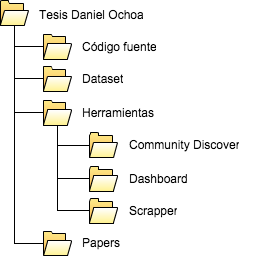
\includegraphics[scale=.5]{images/FiguraB-1}
  \caption{\em Directorios del CD.}
  \label{fig:apb-im1}
\end{figure}

\begin{itemize}
	\item Código fuente: Es una carpeta que contiene el código fuente de RBox 2.0 tal como se puede encontrar en el repositorio de código en bitbucket\footnote{https://bitbucket.org/RodrigoVasquez/recommendation-box}. Es la implementación del \textit{framework} que permite generar sistemas de recomendación en base a la 3-Ontology. La estructura de directorios interna, modo de uso y particularidades de la aplicación pueden encontrarse en el archivo README en la raíz de la carpeta del código fuente.
	\item Dataset: Contiene el \textit{dump} sql de la base de datos de la 3-Ontology que fue utilizada para el análisis. Así mismo, contiene el extenso de los análisis realizados para obtener los resultados.
	\item Herramientas: Contiene todos aquellos componentes desarrollados para complementar el proceso de detección y análisis de comunidades. \newline
	\begin{itemize}
		\item Community Discover: Código del servicio RESTful que permite detectar comunidades. Es una copia fiel del repositorio de código en bitbucket\footnote{https://bitbucket.org/dochoaj/community-discover}. Las instrucciones de uso y precondiciones de instalación están especificadas en el archivo README en la raíz de la carpeta del código fuente.
		\item Dashboard: Código de un dashboard que permite explorar las comunidades detectadas. Es una copia fiel del repositorio de código en bitbucket\footnote{https://bitbucket.org/dochoaj/community-dashboard}. Las instrucciones de uso y precondiciones de instalación están especificadas en el archivo README en la raíz de la carpeta del código fuente.
		\item Scrapper: Código de un scraper que fue utilizado para obtener los datos desde Twitter. Es una copia fiel del repositorio de código en bitbucket\footnote{https://bitbucket.org/dochoaj/3ontology-twitter}. Las instrucciones de uso y precondiciones de instalación están especificadas en el archivo README en la raíz de la carpeta del código fuente.
	\end{itemize}
	\item Papers: Contiene una copia de todos los documentos científicos, a los que fue posible acceder legalmente, y que han sido utilizados como referencia u antecedente de este trabajo de tesis.
\end{itemize} % CD
% \include{chapters/anexo-codigo-1} % Código fuente

\end{document}
